\documentclass[12pt,a3paper]{article}

%% ── Packages ──────────────────────────────────────────────────────────
\usepackage{amsmath,amssymb}
\usepackage{geometry}
\usepackage{enumitem}
\usepackage{titlesec}
\usepackage[hidelinks,colorlinks=true,linkcolor=blue!70!black]{hyperref}
\usepackage{xcolor}
\usepackage{fancyhdr}
\usepackage{tcolorbox}
\usepackage{multicol}
\usepackage{needspace}
\usepackage[strings]{underscore}
\usepackage{array,booktabs}
\usepackage{graphicx}
\usepackage{tikz}
\usepackage{colortbl}
\usepackage{circuitikz}

\tcbuselibrary{skins,breakable}
\geometry{margin=2.5cm,headheight=20pt,top=3cm,bottom=3cm}

%% ── Colors ────────────────────────────────────────────────────────────
\definecolor{pblue}{RGB}{13,71,161}
\definecolor{dgray}{RGB}{66,66,66}
\definecolor{cA}{RGB}{183,28,28}
\definecolor{cB}{RGB}{1,87,155}
\definecolor{cC}{RGB}{27,94,32}
\definecolor{cD}{RGB}{106,27,154}
\definecolor{cE}{RGB}{230,81,0}
\definecolor{cF}{RGB}{0,96,100}
\definecolor{cG}{RGB}{136,14,79}
\definecolor{cH}{RGB}{0,77,64}

%% ── Section & subsection headings ─────────────────────────────────────
\titleformat{\section}{\large\bfseries\color{pblue}}{}{0em}{}[\titlerule]
\titleformat{\subsection}{\normalsize\bfseries}{}{0em}{}
\titlespacing{\subsection}{0pt}{10pt}{4pt}

%% ── Header / Footer ───────────────────────────────────────────────────
\pagestyle{fancy}\fancyhf{}
\renewcommand{\headrulewidth}{0.5pt}
\fancyhead[L]{\small\textcolor{pblue}{\textbf{BUET $|$ PHY 129 Question Bank}}}
\fancyhead[R]{\small\textcolor{dgray}{\textit{\nouppercase{\leftmark}}}}
\fancyfoot[C]{\small\thepage}

%% ── List styles ───────────────────────────────────────────────────────
\setlist[enumerate,1]{label=\textbf{Q\arabic*.},leftmargin=*,itemsep=14pt,parsep=2pt}
\setlist[enumerate,2]{label=(\alph*),leftmargin=2em,itemsep=3pt}
\setlist[enumerate,3]{label=(\roman*),leftmargin=2.5em,itemsep=2pt}

%% ── Utility macros ────────────────────────────────────────────────────
\newcommand{\yr}[1]{\hfill\textcolor{gray}{\small\textbf{[#1]}}}
\newcommand{\mk}[1]{\textcolor{orange!70!black}{\small\textbf{(#1 marks)}}}
\newcommand{\variant}[1]{\par\vspace{1pt}\textcolor{blue!50!black}%
  {\footnotesize\textit{$\hookrightarrow$ Similar: #1}}}

\newcommand{\secdivider}[6]{%
  \newpage\thispagestyle{empty}%
  \vspace*{\fill}%
  \begin{tcolorbox}[enhanced,colback=#6!7,colframe=#5,boxrule=1.5pt,arc=8pt,
    left=20pt,right=20pt,top=22pt,bottom=22pt,
    shadow={3pt}{-3pt}{0pt}{black!15}]
    \centering
    {\large\textcolor{gray}{\textbf{BUET $\cdot$ PHY 129}}}\\[8pt]
    {\fontsize{22}{28}\selectfont\bfseries\textcolor{#5}{#2}}\\[6pt]
    {\fontsize{13}{17}\selectfont\textcolor{dgray}{#3}}\\[10pt]
    \textcolor{#5!60}{\rule{0.5\textwidth}{0.5pt}}\\[6pt]
    {\small\textcolor{gray}{#4}}
  \end{tcolorbox}%
  \vspace*{\fill}\newpage%
}

%% ── Subtopic heading macro ────────────────────────────────────────────
\newcommand{\subtopic}[2]{%
  \vspace{10pt}
  \noindent\begin{tcolorbox}[colback=#1!8,colframe=#1,boxrule=0.6pt,arc=4pt,
    left=6pt,right=6pt,top=4pt,bottom=4pt]
    \small\bfseries\textcolor{#1}{#2}
  \end{tcolorbox}
  \vspace{2pt}
}

%% ── Question environment ──────────────────────────────────────────────
\newcounter{qnum}
\newcommand{\Q}[1]{%
  \needspace{4\baselineskip}
  \refstepcounter{qnum}
  \vspace{6pt}
  \noindent\textbf{Q\theqnum.}\enspace #1\par
}

\begin{document}

%% ══════════════════════════════════════════════════════════════════════
%%  COVER PAGE
%% ══════════════════════════════════════════════════════════════════════
\thispagestyle{empty}
\begin{tcolorbox}[enhanced,colback=pblue!5,colframe=pblue,boxrule=1.5pt,arc=6pt,
  top=28pt,bottom=28pt,left=22pt,right=22pt,
  shadow={4pt}{-4pt}{0pt}{black!20}]
  \centering

  % --- BUET Logo Added Here ---
  
\includegraphics[height=2.5cm]{images/buet_logo.png}\\[8pt]
  % ----------------------------

  {\Large\bfseries\textcolor{pblue}{Bangladesh University of Engineering and Technology}}\\[4pt]
  {\normalsize\textcolor{dgray}{Department of Computer Science \& Engineering}}\\[18pt]
  \textcolor{pblue}{\rule{\textwidth}{1pt}}\\[14pt]

  {\fontsize{22}{28}\selectfont\bfseries\textcolor{pblue}{PHY 129 Question Bank}}\\[8pt]
  {\fontsize{14}{18}\selectfont\textcolor{dgray}{PHY 129 $\cdot$ Structure of Matter, Electricity \& Magnetism,\\ Wave
Mechanics}}\\[4pt]
  \textcolor{pblue}{\rule{\textwidth}{0.5pt}}\\[14pt]

  {\small\textcolor{dgray}{Year Coverage: 2006 to 2024\\
  Topics: Structure of Matter \cdot Electricity \& Magnetism \cdot Wave Mechanics}}\\[16pt]

    {\small\bfseries\textcolor{dgray}{Authors \& Contributors}}\\[6pt]
    \begin{tabular}{rl}
      \textcolor{dgray}{\textbf{Md Ratul Hasan}} \textcolor{dgray}{\small(2405009)} & --- Question Curation \& Organisation\\
      & --- \LaTeX\ Typesetting\\[3pt]
      \textbf{Claude AI}  & --- \LaTeX\ Typesetting\\[3pt]
      \textbf{Gemini}     & --- Diagram Generation\\[3pt]
    \end{tabular}

\end{tcolorbox}
\newpage


%% ── TABLE OF CONTENTS ─────────────────────────────────────────────────
\thispagestyle{fancy}\markboth{Table of Contents}{}
\begin{center}
  {\LARGE\bfseries\textcolor{pblue}{Table of Contents}}\\[6pt]
  \textcolor{pblue}{\rule{0.6\textwidth}{0.8pt}}
\end{center}
\vspace{6pt}

%% Part I
\begin{tcolorbox}[colback=cA!5,colframe=cA,boxrule=1pt,arc=5pt,
  left=8pt,right=8pt,top=8pt,bottom=8pt,before skip=4pt]
  {\large\bfseries\textcolor{cA}{Part I --- Structure of Matter}}\\[5pt]
  \textcolor{cA!40}{\rule{\textwidth}{0.4pt}}\\[3pt]
  \small\begin{itemize}[leftmargin=1.2em,itemsep=1pt,label={\textcolor{cA}{$\triangleright$}}]
    \item \hyperref[sec:s11]{\textbf{S1.1} Crystalline \& Amorphous Solids}
    \item \hyperref[sec:s12]{\textbf{S1.2} Crystal Systems, Crystal Directions \& Unit Cells}
    \item \hyperref[sec:s13]{\textbf{S1.3} Miller Indices \& Interplanar Spacing}
    \item \hyperref[sec:s14]{\textbf{S1.4} Coordination Number \& Packing Factor}
    \item \hyperref[sec:s15]{\textbf{S1.5} Bragg's Law \& X-ray Diffraction}
    \item \hyperref[sec:s16]{\textbf{S1.6} Crystal Structure Analysis}
    \item \hyperref[sec:s17]{\textbf{S1.7} Defects in Crystals}
    \item \hyperref[sec:s18]{\textbf{S1.8} Bonds in Solids, Cohesive \& Bonding Energy}
    \item \hyperref[sec:s19]{\textbf{S1.9} Band Theory of Solids}
    \item \hyperref[sec:s110]{\textbf{S1.10} Solid State Devices}
  \end{itemize}
\end{tcolorbox}

%% Part II
\begin{tcolorbox}[colback=cB!5,colframe=cB,boxrule=1pt,arc=5pt,
  left=8pt,right=8pt,top=8pt,bottom=8pt,before skip=4pt]
  {\large\bfseries\textcolor{cB}{Part II --- Electricity \& Magnetism}}\\[5pt]
  \textcolor{cB!40}{\rule{\textwidth}{0.4pt}}\\[3pt]
  \small\begin{itemize}[leftmargin=1.2em,itemsep=1pt,label={\textcolor{cB}{$\triangleright$}}]
    \item \hyperref[sec:s21]{\textbf{S2.1} Charge, Coulomb's Law \& Ohm's Law}
    \item \hyperref[sec:s22]{\textbf{S2.2} Electric Field}
    \item \hyperref[sec:s23]{\textbf{S2.3} Gauss's Law \& Applications}
    \item \hyperref[sec:s24]{\textbf{S2.4} Electric Potential \& Equipotential Surfaces}
    \item \hyperref[sec:s25]{\textbf{S2.5} Dielectrics \& Electrostatic Energy in Capacitors}
    \item \hyperref[sec:s26]{\textbf{S2.6} Magnetic Field \& Forces}
    \item \hyperref[sec:s27]{\textbf{S2.7} Hall Effect}
    \item \hyperref[sec:s28]{\textbf{S2.8} Biot-Savart \& Amp\`ere's Laws}
    \item \hyperref[sec:s29]{\textbf{S2.9} Electromagnetic Induction \& Inductance}
    \item \hyperref[sec:s210]{\textbf{S2.10} Solenoid and Toroid}
    \item \hyperref[sec:s211]{\textbf{S2.11} RC, LR, LC \& LRC Circuits}
    \item \hyperref[sec:s212]{\textbf{S2.12} Mass Spectrometer}
    \item \hyperref[sec:s213]{\textbf{S2.13} Magnetic Materials \& Computing Applications}
  \end{itemize}
\end{tcolorbox}

%% Part III
\begin{tcolorbox}[colback=cC!5,colframe=cC,boxrule=1pt,arc=5pt,
  left=8pt,right=8pt,top=8pt,bottom=8pt,before skip=4pt]
  {\large\bfseries\textcolor{cC}{Part III --- Wave Mechanics}}\\[5pt]
  \textcolor{cC!40}{\rule{\textwidth}{0.4pt}}\\[3pt]
  \small\begin{itemize}[leftmargin=1.2em,itemsep=1pt,label={\textcolor{cC}{$\triangleright$}}]
    \item \hyperref[sec:s31]{\textbf{S3.1} Failure of Classical Mechanics \& Historical Origins}
    \item \hyperref[sec:s32]{\textbf{S3.2} Wave-Particle Duality}
    \item \hyperref[sec:s33]{\textbf{S3.3} Uncertainty Principle}
    \item \hyperref[sec:s34]{\textbf{S3.4} Postulates of QM \& Wave Function}
    \item \hyperref[sec:s35]{\textbf{S3.5} Operators \& Schr\"odinger Equation}
    \item \hyperref[sec:s36]{\textbf{S3.6} Expectation Value \& Ehrenfest Theorem}
    \item \hyperref[sec:s37]{\textbf{S3.7} Eigenfunction \& Eigenvalues}
    \item \hyperref[sec:s38]{\textbf{S3.8} Particle in a Box}
    \item \hyperref[sec:s39]{\textbf{S3.9} Square Well Potential}
    \item \hyperref[sec:s40]{\textbf{S3.10} Harmonic Oscillator}
  \end{itemize}
\end{tcolorbox}

%% Part IV
\begin{tcolorbox}[colback=cE!5,colframe=cE,boxrule=1pt,arc=5pt,
  left=8pt,right=8pt,top=8pt,bottom=8pt,before skip=4pt]
  {\large\bfseries\textcolor{cE}{Part IV --- Miscellaneous / Not in Syllabus}}\\[5pt]
  \textcolor{cE!40}{\rule{\textwidth}{0.4pt}}\\[3pt]
  \small\begin{itemize}[leftmargin=1.2em,itemsep=1pt,label={\textcolor{cE}{$\triangleright$}}]
    \item \hyperref[sec:s4a]{\textbf{S4a.} Heat \& Thermodynamics}
    \item \hyperref[sec:s4b]{\textbf{S4b.} Physical Optics}
    \item \hyperref[sec:s4c]{\textbf{S4c.} Waves \& Oscillation}
  \end{itemize}
\end{tcolorbox}

\newpage

%% ══════════════════════════════════════════════════════════════════════
%%  PART I: STRUCTURE OF MATTER
%% ══════════════════════════════════════════════════════════════════════
\secdivider{Part I}{Structure of Matter}%
  {Crystal Systems, Bonding, Defects, Band Theory, Solid State Devices}%
  {Crystalline \& amorphous solids $\cdot$ Crystal systems $\cdot$ Crystal directions $\cdot$ Miller indices $\cdot$ Coordination number $\cdot$ Packing factor $\cdot$ Bragg's law $\cdot$ Crystal structure analysis $\cdot$ Defects $\cdot$ Bonds $\cdot$ Cohesive energy $\cdot$ Free electron theory $\cdot$ Band theory $\cdot$ Solid state devices}%
  {cA}{red}

\markboth{Part I: Structure of Matter}{Part I: Structure of Matter}
\label{sec:S1}
\section*{Part I \quad Structure of Matter}
\addcontentsline{toc}{section}{Part I: Structure of Matter}

%% ── S1.1 ──────────────────────────────────────────────────────────────
\label{sec:s11}
\subtopic{cA}{S1.1 \quad Crystalline and Amorphous Solids}

\begin{enumerate}

\item Explain how solids are classified from a crystallographic perspective. How do
cubic and orthorhombic crystal systems differ in terms of their structural
characteristics?
\mk{10} \yr{PHY 129 | L-1/T-1 | 2024-25}

\item Distinguish between cubic and hexagonal crystal systems. Draw the unit cells of various space lattices and calculate the number of atoms per unit cell in various space lattices of these crystal systems.
\mk{11} \yr{PHY 129 | L-1/T-1 | 2023-24}

\item Distinguish between cubic and hexagonal crystal systems. Draw the unit cells of various space lattices and calculate the number of atoms per unit cell in various space lattices of these crystal systems.
\mk{11} \yr{PHY 129 | L-1/T-1 | 2023-24}

\item Discuss the classification of solids from the crystallographic point of view. Distinguish between cubic and orthorhombic crystal systems.
\mk{11} \yr{PHY 129 | L-1/T-1 | 2022-23}
\variant{PHY 109 | 2013-14}

\item Discuss the classification of solids from the crystallographic point of view. Distinguish between cubic and orthorhombic crystal systems.
\mk{11} \yr{PHY 129 | L-1/T-1 | 2022-23}
\variant{PHY 109 | 2013-14}

\item Illustrate unit cells for various space lattices in orthorhombic and cubic crystal systems. Compare the atomic radii, number of atoms per cell, and coordination number of various space lattices in the cubic crystal system.
\mk{20} \yr{PHY 129 | L-1/T-1 | 2021-22}


\item Distinguish between crystalline and amorphous solids. Among them which is more stable and why? Explain allotropy with some examples. What is graphene?
\mk{part} \yr{PHY 109 | L-1/T-1 | 2014-15}
\variant{PHY 109 | 2006-07; PHY 109 | 2011-12}

\item Explain polymorphism with some examples. What is graphene?
\mk{10} \yr{PHY 109 | L-1/T-1 | 2011-12}

\item Describe the difference in atomic/molecular structure between crystalline and non-crystalline materials.
\mk{8} \yr{PHY 109 | L-1/T-1 | 2008-09}
\variant{PHY 129 | 2021-22}

\item Distinguish clearly between crystalline and amorphous solids. Of these two states, which is more thermodynamically favourable and why?
\mk{11} \yr{PHY 109 | L-1/T-1 | 2006-07}
\variant{PHY 109 | 2011-12}

\end{enumerate}
%% ── S1.2 ──────────────────────────────────────────────────────────────
\label{sec:s12}
\subtopic{cA}{S1.2 \quad Crystal Systems, Crystal Directions \& Unit Cells}

\begin{enumerate}

\item Draw all three-dimensional Bravais lattices associated with the cubic and
orthorhombic crystal systems. Derive the mathematical relationship between the
atomic radius and lattice constant for the cubic crystal structures.
\mk{15} \yr{PHY 129 | L-1/T-1 | 2024-25}


\item Draw typical unit cells for Lithium (Li) and Copper (Cu) crystals. Derive the relationship between atomic radii and lattice constants for Li and Cu crystals. Find out the percentage of interatomic spaces of these crystals.
\mk{11} \yr{PHY 129 | L-1/T-1 | 2023-24}

\item A metal crystallizes in a simple cubic structure with an edge length of $0.328$~nm. What is the radius of the metal atom?
\mk{part} \yr{PHY 129 | L-1/T-1 | 2023-24}

\item Sketch all 3D Bravais lattices of cubic and orthorhombic crystal systems. Formulate relationships between atomic radii and lattice parameters for the cubic crystal system.
\mk{14} \yr{PHY 129 | L-1/T-1 | 2022-23}
\variant{PHY 109 | 2013-14}

\item Illustrate a typical unit cell of a hexagonal close-packed crystal. Evaluate the $c/a$ ratio for this type of crystal.
\mk{10} \yr{PHY 129 | L-1/T-1 | 2022-23}
\variant{PHY 109 | 2012-13; PHY 109 | 2014-15}

\item Illustrate a typical unit cell of hexagonal close-packed (HCP) crystal structure. Cite some examples of HCP crystal. Compute the number of atoms per unit cell of an HCP crystal structure.
\mk{part} \yr{PHY 129 | L-1/T-1 | 2021-22}

\item Niobium (Nb) is BCC with a density of $8.57\ \text{g/cm}^3$. (i) Calculate the centre-to-centre distance between the closest atoms. (ii) What is the edge dimension of the unit cell? Given: $M_{\text{Nb}} = 92.91\ \text{g/mol}$.
\mk{8} \yr{PHY 129 | L-1/T-1 | 2021-22}

\item What are the lattice parameters of a 3D unit cell? Mention lattice parameters of hexagonal crystal system. Give some examples of hexagonal crystals. Draw a typical 3D unit cell for hexagonal crystal, calculate number of atoms per unit cell and coordination number. Show that for an ideal hexagonal crystal the $c/a$ ratio is $1.633$.
\mk{part} \yr{PHY 109 | L-1/T-1 | 2014-15}
\variant{PHY 109 | 2012-13}

\item Calculate the number of atoms per unit cell in various space lattices of the cubic crystal system. Provide necessary diagrams.
\mk{part} \yr{PHY 109 | L-1/T-1 | 2014-15}

\item What is the crystalline nature of $\alpha$-iron? The atomic radius of $\alpha$-iron is $0.1243$~nm. Calculate the lattice constant and density of $\alpha$-iron.
\mk{6.5} \yr{PHY 109 | L-1/T-1 | 2013-14}

\item Write down the lattice parameters for orthorhombic and cubic crystal systems. Draw the unit cells for various space lattices in orthorhombic and cubic crystal systems.
\mk{16} \yr{PHY 109 | L-1/T-1 | 2012-13}

\item Draw a schematic diagram of a unit cell for the 3D hexagonal crystal system. Calculate the $c/a$ ratio for this crystal system. Give some examples of hexagonal crystals.
\mk{16} \yr{PHY 109 | L-1/T-1 | 2012-13}

\item The KCl crystal is FCC with density $1.98\ \text{g/cm}^3$ and molecular weight $74.6$~g/mol. Calculate (i) the distance from one atom to the next atom of the same kind and (ii) the distance between adjacent atoms.
\mk{5.5} \yr{PHY 109 | L-1/T-1 | 2012-13}

\item What are the lattice parameters of a 3D unit cell? What are Bravais lattices and crystal systems? Mention all 3D Bravais lattices with their crystal system and lattice parameters.
\mk{20} \yr{PHY 109 | L-1/T-1 | 2011-12}

\item Unit cell edge length of gold crystal is $0.4080$~nm. How many unit cells are in a gold foil of length $2$~cm, breadth $2$~cm and thickness $0.02$~mm?
\mk{3.5} \yr{PHY 109 | L-1/T-1 | 2011-12}

\item What is space lattice? Write down the unit cell characteristics of the seven crystal systems with fourteen Bravais lattices.
\mk{part} \yr{PHY 109 | L-1/T-1 | 2010-11}

\item Draw the unit cell of diamond crystal and find the number of atoms per cell.
\mk{part} \yr{PHY 109 | L-1/T-1 | 2010-11}

\item Draw unit cells for FCC, BCC, and HCP crystal structures and calculate the number of atoms per unit cell.
\mk{15} \yr{PHY 109 | L-1/T-1 | 2008-09}

\item Derive the relationships between unit cell edge length and atomic radius for FCC and BCC crystal structures.
\mk{15} \yr{PHY 109 | L-1/T-1 | 2008-09}
\variant{PHY 109 | 2011-12; PHY 109 | 2013-14}

\item A hypothetical metal has the simple cubic crystal structure. If its atomic weight is $74.5$~g/mol and the atomic radius is $0.145$~nm, compute its density.
\mk{part} \yr{PHY 109 | L-1/T-1 | 2008-09}

\item What is a unit cell? What are the lattice parameters of a unit cell?
\mk{8} \yr{PHY 109 | L-1/T-1 | 2006-07}

\item The experimental density of single-crystal Al is $2.697\ \text{g/cm}^3$ with lattice constant $a = 0.4049\times10^{-9}$~m. If the discrepancy between calculated and experimental density results from vacancies, (i) what fraction of atom sites are vacant? (ii) how many vacancies are there per cm$^3$?
\mk{8.5} \yr{PHY 109 | L-1/T-1 | 2006-07}

\item Explain space lattice and basis of a crystal.
\mk{10} \yr{PHY 109 | L-1/T-1 | 2005-06}
\variant{PHY 109 | 2012-13}

\item Derive an expression for calculating the theoretical density of a crystalline solid. Write down the expression for SC, BCC, and FCC structures.
\mk{14} \yr{PHY 109 | L-1/T-1 | 2005-06}

\item Write down the lattice parameters for a hexagonal lattice. Show that the $c/a$ ratio for an ideal HCP lattice is $1.633$. Using this relation estimate the packing fraction of HCP crystal.
\mk{12} \yr{PHY 109 | L-1/T-1 | 2005-06}
\variant{PHY 109 | 2010-11}

\item A gold foil is $67$~mm long, $10$~mm wide and $0.08$~mm thick. Gold crystallises in a cubic structure with lattice constant $a = 0.4076\times10^{-6}$~mm. (i) How many unit cells are there in the foil? (ii) What is the mass of each unit cell if the density is $19.32\ \text{g/cm}^3$?
\mk{10.5} \yr{PHY 109 | L-1/T-1 | 2005-06}

\end{enumerate}
%% ── S1.3 ──────────────────────────────────────────────────────────────
\label{sec:s13}
\subtopic{cA}{S1.3 \quad Miller Indices \& Interplanar Spacing}

\begin{enumerate}
\item Derive a mathematical expression that relates the interplanar spacing $d_{hkl}$ to the
Miller indices for a crystal belonging to the orthorhombic system.
\mk{15} \yr{PHY 129 | L-1/T-1 | 2024-25}


\item Sketch $[100]$, $[110]$, and $[111]$ crystal directions in a unit cell of a typical BCC crystal. What is the linear density of atoms? Compute and compare linear density values for $\alpha$-Fe in these directions. Atomic radius of Fe is $0.1243$~nm.
\mk{14} \yr{PHY 129 | L-1/T-1 | 2023-24}
\variant{PHY 109 | 2013-14}

\item Sketch $(100)$, $(110)$ and $(111)$ crystal planes in a unit cell of a typical FCC crystal. What is the planar density of atoms? Compute and compare the planar density for these planes for silver (Ag) crystal. Atomic radius of Ag is $0.144$~nm.
\mk{14} \yr{PHY 129 | L-1/T-1 | 2023-24}
\variant{PHY 109 | 2013-14}

\item Deduce an expression relating the Miller indices and interplanar distance for an orthorhombic crystal system.
\mk{14} \yr{PHY 129 | L-1/T-1 | 2022-23}

\item Calculate the wavelength of X-rays that are diffracted at $43.4^\circ$ by copper crystal, whose lattice constant is $0.3615$~nm. This diffraction peak for copper is the first order for $d_{111}$. Illustrate a typical unit cell of copper crystal.
\mk{10} \yr{PHY 129 | L-1/T-1 | 2022-23}

\item What are the Miller indices? How will you find the Miller indices? Show that the Miller indices and interplanar distance are related for a cubic crystal system by $d = a/\sqrt{h^2+k^2+l^2}$.
\mk{20} \yr{PHY 129 | L-1/T-1 | 2021-22}
\variant{PHY 109 | 2006-07; PHY 109 | 2012-13}

\item Lead (Pb) crystal is FCC with an atomic radius of $0.1750$~nm. Illustrate $(100)$ and $(110)$ crystal planes of Pb crystal. Compute the planar density of atoms in the $(110)$ plane.
\mk{8} \yr{PHY 129 | L-1/T-1 | 2021-22}

\item Sketch $[100]$, $[110]$ and $[111]$ crystal directions in a unit cell of a typical FCC crystal. What is linear density of atoms? Compute linear density values for these crystal directions.
\mk{part} \yr{PHY 109 | L-1/T-1 | 2013-14}

\item Sketch $(100)$, $(110)$ and $(111)$ crystal planes in a unit cell of a typical BCC crystal. What is planar density of atoms? Compute planar density values for these planes for $\alpha$-iron crystal.
\mk{12} \yr{PHY 109 | L-1/T-1 | 2013-14}

\item Draw the $(100)$, $(011)$, $(101)$ and $(010)$ planes for a simple cubic structure.
\mk{part} \yr{PHY 109 | L-1/T-1 | 2010-11}
\variant{PHY 109 | 2007-08}

\item Draw the $(112)$, $(001)$ and $(110)$ crystal planes in a simple cubic crystal.
\mk{10} \yr{PHY 109 | L-1/T-1 | 2007-08}

\item Show that in a crystal of cubic structure, the interplanar distance between planes with Miller indices $(hkl)$ is equal to $d = a/\sqrt{h^2+k^2+l^2}$.
\mk{15} \yr{PHY 109 | L-1/T-1 | 2006-07}
\variant{PHY 109 | 2012-13}

\item Aluminium crystal is FCC with atomic radius $r = 0.1432\times10^{-9}$~m. Calculate the interplanar distances for the $(200)$, $(220)$, and $(111)$ planes. (Assume atoms are hard spheres.)
\mk{12.5} \yr{PHY 109 | L-1/T-1 | 2006-07}

\end{enumerate}

%% ── S1.4 ──────────────────────────────────────────────────────────────
\label{sec:s14}
\subtopic{cA}{S1.4 \quad Coordination Number \& Packing Factor}

\begin{enumerate}

\item Depict a typical unit cell of hexagonal close-packed (HCP) structure. Calculate
the coordination number of atoms per unit cell for this structure. Derive the ratio
of the lattice constants \textbf{c/a} for this crystal structure.  
\mk{10} \yr{PHY 129 | L-1/T-1 | 2024-25}


\item What is packing factor? Calculate packing factor for BCC and FCC crystals.
\mk{16} \yr{PHY 129 | L-1/T-1 | 2012-13}
\variant{PHY 109 | 2007-08}

\item (i) Draw typical unit cells of NaCl and CsCl crystals. (ii) Describe their crystal structure. (iii) Calculate their packing factors. [Given $R_{\text{Na}^+} = 0.097$~nm, $R_{\text{Cs}^+} = 0.187$~nm, $R_{\text{Cl}^-} = 0.169$~nm]
\mk{16} \yr{PHY 109 | L-1/T-1 | 2012-13}

\item Define coordination number. What are the coordination numbers of (i) simple cubic, (ii) body-centred cubic, and (iii) face-centred cubic crystals? Explain with the help of neat sketches.
\mk{10} \yr{PHY 109 | L-1/T-1 | 2011-12}
\variant{PHY 109 | 2013-14}

\item What is the crystalline nature of nickel? Sketch the $(100)$ plane of the nickel crystal. Atomic radius of nickel is $0.1248$~nm. (i) What is the area of this plane? (ii) Calculate the number of atoms/mm$^2$ of the $(100)$ plane. Calculate the packing factor for nickel crystal.
\mk{6.5} \yr{PHY 109 | L-1/T-1 | 2011-12}

\item What do you understand by the packing factor of a crystal? Obtain the expressions for packing factors for sodium (BCC) and copper (FCC) crystals.
\mk{21.5} \yr{PHY 109 | L-1/T-1 | 2007-08}

\end{enumerate}
%% ── S1.5 ──────────────────────────────────────────────────────────────
\label{sec:s15}
\subtopic{cA}{S1.5 \quad Bragg's Law \& X-ray Diffraction}

\begin{enumerate}

\item Define X-ray diffraction in the context of crystallography. What key structural
insights can be obtained from the X-ray diffraction analysis of a crystal?
\mk{10} \yr{PHY 129 | L-1/T-1 | 2024-25}

\item Sketch and describe the unit cell structure of gold, identifying its crystal type. Copper exhibits a diffraction peak at an angle of $2\theta= 42.8^o$, corresponding to the first-order reflection from the (1 1 1) planes. Given that the lattice constant of gold is 0.407nm, calculate the wavelength of the incident X-rays.
\mk{10} \yr{PHY 129 | L-1/T-1 | 2024-25}



\item Describe X-ray diffraction related to crystallography. What information do you get from X-ray diffraction of a crystal? Deduce an expression relating the Miller indices and interplanar distance for an orthorhombic crystal system.
\mk{25} \yr{PHY 129 | L-1/T-1 | 2022-23}
\variant{PHY 109 | 2005-06}

\item Describe X-ray diffraction related to crystallography. What information do you get from X-ray diffraction of a crystal?
\mk{11} \yr{PHY 129 | L-1/T-1 | 2022-23}

\item Draw a schematic diagram of an X-ray diffractometer. Deduce Bragg's law. Draw a typical X-ray diffraction pattern for body-centred cubic polycrystalline iron with their Miller indices.
\mk{20} \yr{PHY 109 | L-1/T-1 | 2014-15}

\item Determine the first-order diffraction angle through which an X-ray of wavelength $0.44$~\AA\ is reflected from the $(102)$ plane of a simple cubic crystal having lattice constant $2.42$~\AA.
\mk{10} \yr{PHY 109 | L-1/T-1 | 2010-11}

\item The Bragg angle for reflection from the $(111)$ planes in aluminium (FCC) is $19.2^\circ$ for an X-ray wavelength of $1.54$~\AA. Compute (i) the cube edge of the unit cell and (ii) the interplanar distance for these planes.
\mk{10} \yr{PHY 109 | L-1/T-1 | 2007-08}

\item Derive Bragg's law of X-ray diffraction. Draw a schematic diagram of a typical X-ray diffractometer.
\mk{12} \yr{PHY 109 | L-1/T-1 | 2005-06}
\variant{PHY 109 | 2007-08; PHY 109 | 2010-11}

\end{enumerate}
%% ── S1.6 ──────────────────────────────────────────────────────────────
\label{sec:s16}
\subtopic{cA}{S1.6 \quad Crystal Structure Analysis}

\begin{enumerate}

\item Define Wigner--Seitz primitive cell.
\mk{part} \yr{PHY 109 | L-1/T-1 | 2010-11}

\item Draw and explain the unit cell of NaCl crystal.
\mk{15} \yr{PHY 109 | L-1/T-1 | 2007-08}

\end{enumerate}

%% ── S1.7 ──────────────────────────────────────────────────────────────
\label{sec:s17}
\subtopic{cA}{S1.7 \quad Defects in Crystals}

\begin{enumerate}

\item What are crystal defects? Briefly describe the different types of defects commonly observed in crystalline solids.
\mk{10} \yr{PHY 129 | L-1/T-1 | 2024-25}


\item Suppose the energy required to form a vacancy in tungsten (W) crystal is $1.3$~eV, and the density of W is $19280\ \text{kg/m}^3$. Evaluate the equilibrium number of vacancies per cubic metre in W crystal at $1050^\circ$C.
\mk{part} \yr{PHY 129 | L-1/T-1 | 2023-24}
\variant{PHY 129 | 2022-23}

\item Briefly analyse the statement ``Real crystals are never perfect''.
\mk{11} \yr{PHY 129 | L-1/T-1 | 2022-23}

\item Describe the classification of defects observed in solids. Obtain an expression for the Schottky defect for a typical metal.
\mk{14} \yr{PHY 129 | L-1/T-1 | 2022-23}
\variant{PHY 109 | 2006-07; PHY 109 | 2012-13}

\item Consider the energy required to form a vacancy in copper crystal is $0.9$~eV and the density of copper is $8960\ \text{kg/m}^3$. Evaluate the equilibrium number of vacancies in $1\ \text{m}^3$ of copper crystal at $1050^\circ$C.
\mk{10} \yr{PHY 129 | L-1/T-1 | 2022-23}

\item What are crystal effects? Explain briefly various types of defects in a solid.
\mk{7} \yr{PHY 129 | L-1/T-1 | 2022-23} 

\item What is dislocation? Describe edge dislocation and screw dislocation.
\mk{21.5} \yr{PHY 109 | L-1/T-1 | 2007-08}

\item Briefly explain the different types of defects that exist in solids.
\mk{12} \yr{PHY 109 | L-1/T-1 | 2006-07}
\variant{PHY 109 | 2012-13}

\item A few defects in crystals are demanded by nature --- discuss this statement from a thermodynamic point of view.
\mk{10} \yr{PHY 109 | L-1/T-1 | 2005-06}

\end{enumerate}

%% ── S1.8 ──────────────────────────────────────────────────────────────
\label{sec:s18}
\subtopic{cA}{S1.8 \quad Bonds in Solids, Cohesive \& Bonding Energy}

\begin{enumerate}

\item Briefly describe the different types of interatomic bonds that exist in solid
materials.   \mk{10} \yr{PHY 129 | L-1/T-1 | 2024-25}


\item Why do interatomic or intermolecular bonds exist in solids? Why is the study of bonds in solids important for a Computer Engineer? Distinguish between primary and secondary bonds.
\mk{11} \yr{PHY 129 | L-1/T-1 | 2023-24}
\variant{PHY 109 | 2011-12; PHY 109 | 2013-14}

\item Distinguish between lattice energy and cohesive energy of an ionic crystal. Draw a typical unit cell of KCl crystal. Find an expression for the lattice energy of the KCl crystal.
\mk{11} \yr{PHY 129 | L-1/T-1 | 2023-24}
\variant{PHY 109 | 2011-12}

\item The ionization energy of potassium (K) is $4.34$~eV and the electron affinity of chlorine (Cl) is $3.6$~eV. The Madelung constant for KCl is $1.748$ and the distance between ions of opposite sign is $0.314$~nm; if $n = 9$, calculate the cohesive energy for the KCl crystal.
\mk{part} \yr{PHY 129 | L-1/T-1 | 2023-24}

\item Explain the term cohesive energy of an ionic crystal. Derive an expression for the cohesive energy of NaCl crystal.
\mk{20} \yr{PHY 129 | L-1/T-1 | 2021-22}
\variant{PHY 109 | 2005-06; PHY 109 | 2008-09; PHY 109 | 2011-12}

\item Show that for an ionic crystal the lattice energy is given by $U = -\frac{N A e^2}{4\pi\varepsilon_0 r_0}\left(1 - \frac{1}{n}\right)$, where the symbols have their usual meaning.
\mk{15} \yr{PHY 109 | L-1/T-1 | 2013-14}

\item Distinguish between lattice energy and cohesive energy of an ionic crystal. Derive an expression for lattice energy for a typical ionic crystal.
\mk{20} \yr{PHY 109 | L-1/T-1 | 2011-12}

\item Explain the following terms: (i) Ionization energy, (ii) Electron affinity, (iii) Cation, and (iv) Anion.
\mk{8} \yr{PHY 109 | L-1/T-1 | 2008-09}

\item What are the characteristics of primary bonds in solids? Explain the various types of primary bonds.
\mk{13} \yr{PHY 109 | L-1/T-1 | 2006-07}
\variant{PHY 109 | 2008-09}

\item Explain the type of bond that exists in an NaCl crystal.
\mk{6.5} \yr{PHY 109 | L-1/T-1 | 2005-06}

\end{enumerate}


%% ── S1.10 ─────────────────────────────────────────────────────────────
\label{sec:s19}
\subtopic{cA}{S1.9 \quad Band Theory of Solids}

\begin{enumerate}

\item Explain the terms valence band, conduction band and energy gap. Using band
theory, illustrate the energy band diagrams for metals, insulators and extrinsic
semiconductors.  \mk{15} \yr{PHY 129 | L-1/T-1 | 2024-25}


\item Illustrate the band diagrams for metal, insulator, and extrinsic semiconductors.
\mk{part} \yr{PHY 129 | L-1/T-1 | 2021-22}
\variant{PHY 109 | 2006-07; PHY 109 | 2010-11}

\item Explain metals, semiconductors, and dielectrics by means of band theory.
\mk{part} \yr{PHY 109 | L-1/T-1 | 2010-11}
\variant{PHY 109 | 2006-07}

\item A solid is found to have an energy band gap of $3$~eV. What is the likely colour of this solid in transmitted sunlight?
\mk{part} \yr{PHY 109 | L-1/T-1 | 2008-09}

\item Distinguish between metals, insulators, and semiconductors according to the band theory of solids.
\mk{part} \yr{PHY 109 | L-1/T-1 | 2006-07}
\variant{PHY 109 | 2010-11}

\end{enumerate}

%% ── S1.11 ─────────────────────────────────────────────────────────────
\label{sec:s110}
\subtopic{cA}{S1.10 \quad Solid State Devices}

\begin{enumerate}

\item What are intrinsic and extrinsic semiconductors? Mention common methods of fabricating extrinsic semiconductors and write an expression for the mobility of an extrinsic semiconductor.
\mk{part} \yr{PHY 109 | L-1/T-1 | 2006-07}

\end{enumerate}


%% ══════════════════════════════════════════════════════════════════════
%%  PART II: ELECTRICITY AND MAGNETISM
%% ══════════════════════════════════════════════════════════════════════
\secdivider{Part II}{Electricity \& Magnetism}%
  {Electrostatics, Magnetostatics, Electromagnetic Oscillations}%
  {Electric field $\cdot$ Gauss's law $\cdot$ Electric potential $\cdot$ Dielectrics $\cdot$ Magnetic field $\cdot$ Hall effect $\cdot$ Biot-Savart \& Amp\`ere's laws $\cdot$ EM induction $\cdot$ Energy in magnetic field $\cdot$ RC/LR/LC/LRC circuits $\cdot$ Transformers $\cdot$ Motors \& generators $\cdot$ Magnetic materials}%
  {cB}{blue}

\markboth{Part II: Electricity \& Magnetism}{Part II: Electricity \& Magnetism}
\label{sec:S2}
\section*{Part II \quad Electricity \& Magnetism}
\addcontentsline{toc}{section}{Part II: Electricity \& Magnetism}


\label{sec:s21}
\subtopic{cA}{S2.1 \quad Charge, Coulomb's Law \& Ohm's Law}

\begin{enumerate}

\item Show that for a conductor obeying Ohm's law the electrical conductivity can be given $\sigma = \frac{nq^2\tau}{m_e}$, where the symbols have their usual meanings.
\mk{5} \yr{PHY 129 | L-1/T-1 | 2024-25}

\item What do you mean by electrical resistivity? Briefly describe the effect of temperature on the resistivity of a metal.
\mk{10} \yr{PHY 129 | L-1/T-1 | 2022-23}

\end{enumerate}


\label{sec:s22}
\subtopic{cA}{S2.2 \quad Electric Field}

\begin{enumerate}

  \item A ring of radius $R$ carries a uniformly distributed positive total charge $Q$ as shown below.
    \begin{enumerate}
        \item[(i)] Calculate the electric field due to the ring at a point $P$ lying a distance $Z$ from its center along the central axis perpendicular to the plane of the ring.
        
        \item[(ii)] Find the position on the axis at which the electric field has the maximum value. What is the maximum value of the electric field at that point?
        
        \item[(iii)] A negatively charged particle $-q$ is placed at the center of the uniformly charged ring, which is confined to move along the $z$ axis, is displaced a small distance $z$ along the axis (where $z \ll R$) and released. Show that the particle oscillates in simple harmonic motion. Find the frequency of the oscillation.
    \end{enumerate}

\begin{center}
  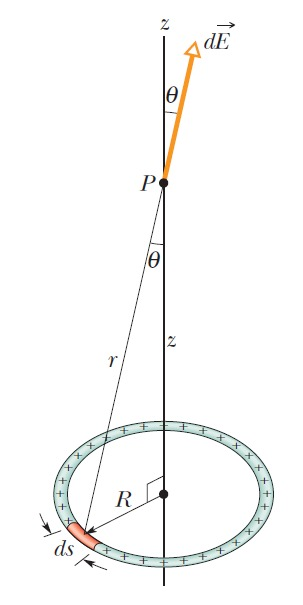
\includegraphics[height=0.4\textheight, width=0.75\textwidth,keepaspectratio]{images/ring.png}
\end{center}
\mk{7+5+8} \yr{PHY 129 | L-1/T-1 | 2024-25}

\item Write short notes on (i) Hall effect and (ii) Gaussian surface.
\mk{10} \yr{PHY 129 | L-1/T-1 | 2022-23}

\item Derive an expression for electric field $E$ at a distance $r$ from the centre of a charged ring having a net charge $Q$ on it.
\mk{10} \yr{PHY 129 | L-1/T-1 | 2022-23}

\item A cube-like Gaussian surface encloses a net charge of $+2Q\varepsilon_0$ and lies in an electric field $\vec{E} = 2x\hat{i} + 9\hat{j} - Bz\hat{k}$ with $x$ and $z$ in metres and $B$ a constant. If the edge length of the cube is $3.00$~m, what is the value of $B$?
\begin{center}
  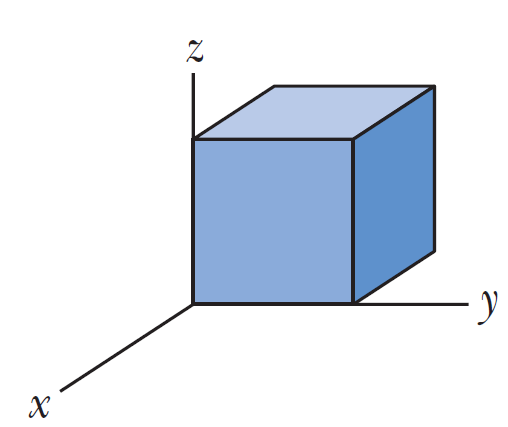
\includegraphics[height=0.2\textheight, width=0.75\textwidth,keepaspectratio]{images/box2.png}
\end{center}

\mk{10} \yr{PHY 129 | L-1/T-1 | 2022-23}

\item Define electric dipole. Estimate the amount of energy stored in an electric dipole placed in an external electric field $E$.
\mk{12} \yr{PHY 129 | L-1/T-1 | 2021-22}

\item A closed Gaussian surface is a cube of edge length $3.0$~m with one corner at $x_1 = 5.00$~m, $y_1 = 4.00$~m. The electric field vector is $\vec{E} = 3x\hat{i} - 4y^2\hat{j} + 5\hat{k}$, where $x$ and $y$ are in metres. What is the net charge contained by the cube?
\mk{10} \yr{PHY 129 | L-1/T-1 | 2021-22}

\begin{center}
  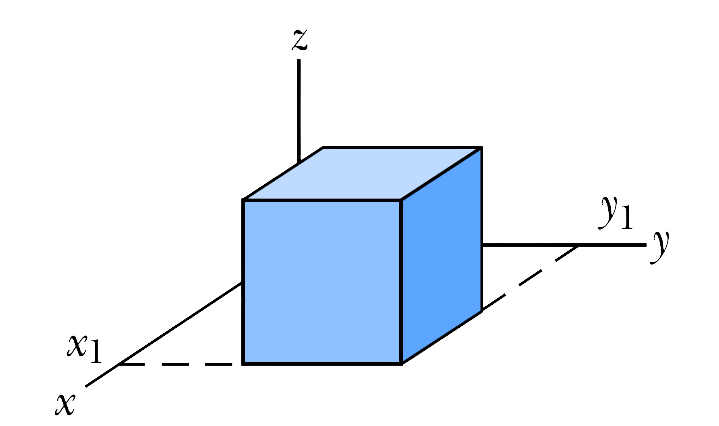
\includegraphics[height=0.2\textheight, width=0.75\textwidth,keepaspectratio]{images/box.png}
\end{center}

\item Prove that the electric field intensity due to an electric dipole at a point on the axial line is double the electric field intensity at a point on the equatorial line. Also find the direction of electric field intensity in both cases.
\mk{20.5} \yr{PHY 109 | L-1/T-1 | 2020-21}

\item Derive an expression for the potential energy of an electric dipole placed in a uniform external electric field. Draw the corresponding energy graph and give a brief explanation.
\mk{14} \yr{PHY 109 | L-1/T-1 | 2020-21}

\item 
    \begin{enumerate}
        \item The Wheatstone bridge shown below has four resistors, three of equal resistance $R_1 = R_3 = R_4 = 10\,\Omega$ and one temperature-varying platinum resistor $R_T$. A voltage $V_{in} = 1\,\text{V}$ is provided to the system by a battery as shown. $V_o$ is defined as the voltage difference between points a and b, and is given by the general Wheatstone bridge equation, 
        \[
        V_o = V_{in}\left(\frac{R_4}{R_1+R_4} - \frac{R_3}{R_T+R_3}\right)
        \]
        Resistance $R_T$ is given by $R_T = R_o[1 - \alpha(T - T_o)]$, where $\alpha$ is the temperature coefficient of platinum, $\alpha = 0.00385\,/^\circ\text{C}$. Given that $R_o = 10\,\Omega$ and $T_o = 0^\circ\text{C}$.
        
        \vspace{0.5cm}
        \noindent\textit{Explain why the platinum is used in platinum resistance thermometer instead of other metals? Write an equation for $V_o$ in terms of $T$.} \mk{15}

        
        
        \item Find $V_o$ at $T = 20^\circ\text{C}$, $T = 30^\circ\text{C}$, $T = 40^\circ\text{C}$, and $T = 50^\circ\text{C}$. Plot a graph with $V_o$ as ordinate and $T$ as abscissa. Find the $V_o$ that would be expected at $T = 37^\circ\text{C}$.\mk{25}
    \end{enumerate}
    \begin{center}
    \begin{circuitikz}[thick,scale=1.2, transform shape]
    
    % Define coordinate points for the corners of the bridge
    \coordinate (top) at (0, 2);
    \coordinate (bottom) at (0, -2);
    \coordinate (left) at (-3, 0);
    \coordinate (right) at (3, 0);

    % Draw the bridge components (resistors)
    \draw (left) to[R, l=$R_1$] (top);
    \draw (top) to[R, l=$R_T$] (right);
    \draw (left) to[R, l_=$R_3$] (bottom);
    \draw (bottom) to[R, l_=$R_4$] (right);

    % Draw the input voltage source and its connecting wires
    \draw (-4.5, 2) -- (top);
    \draw (-4.5, -2) -- (bottom);
    \draw (-4.5, 2) to[battery1, l_=$V_{in}$] (-4.5, -2);

    % Draw the output voltage terminals in the center
    \draw (left) to[short, -o] (-0.6, 0);
    \draw (right) to[short, -o] (0.6, 0);
    \node at (0, 0) {$V_o$};

    % Add node labels 'a' and 'b'
    \node[left] at (left) {$a$};
    \node[right] at (right) {$b$};

\end{circuitikz}
\end{center}
\yr{PHY 109 | L-1/T-1 | Jan 2020}

\item What do you mean by electric charge? What are the basic properties of electric charge? Explain the terms (i) quantization and (ii) conservation of charge.
\mk{13} \yr{PHY 109 | L-1/T-1 | 2016-17}

\item An electric dipole is placed in a uniform external electric field. Find the expression for the torque exerted on the dipole and the work needed to change the orientation of the dipole by an angle $\theta$.
\mk{16} \yr{PHY 109 | L-1/T-1 | 2016-17}

\end{enumerate}

\label{sec:s23}
\subtopic{cA}{S2.3 \quad Gauss's Law \& Applications}

\begin{enumerate}

\item A uniformly charged conducting sphere of $160$~cm diameter has a surface charge density of $7.6\ \mu\text{C/m}^2$. (i) Find the net charge on the sphere. (ii) What is the total electric flux leaving the surface?
\mk{12} \yr{PHY 109 | L-1/T-1 | 2020-21}

\item A solid non-conducting sphere of radius $R$ has a total charge $Q$. Find the electric potential both inside and outside the sphere. Draw schematically the electric potential as a function of distance from the centre.
\mk{22.5} \yr{PHY 109 | L-1/T-1 | 2018-19}

\item Explain the terms electric flux and solid angle. Derive Gauss's law of electrostatics for an isolated point charge $Q$.
\mk{12} \yr{PHY 109 | L-1/T-1 | 2017-18}

\item Discuss the advantages of Gauss's law over Coulomb's law. Deduce Coulomb's law from Gauss's law.
\mk{12} \yr{PHY 109 | L-1/T-1 | 2017-18}

\item Using Gauss's law, calculate $E$ for an infinitely long line of charge with constant charge per unit length $\lambda$.
\mk{12.5} \yr{PHY 109 | L-1/T-1 | 2017-18}

\item An $\alpha$-particle, approaching the surface of a gold nucleus, is at a distance equal to one nuclear radius ($6.9\times10^{-15}$~m) from that surface. What are the forces on the $\alpha$-particle and its acceleration at that point? Mass of $\alpha$-particle $= 6.7\times10^{-27}$~kg.
\mk{10} \yr{PHY 109 | L-1/T-1 | 2017-18}

\item State Gauss's law of electrostatics. Using Gauss's law, calculate the electric field $E$ for a uniformly charged solid sphere of radius $a$ at a distance $r$ from the centre (charge $Q$) for the cases (i) $r>a$, (ii) $r=a$, and (iii) $r<a$.
\mk{16} \yr{PHY 109 | L-1/T-1 | 2015-16}


\end{enumerate}


\label{sec:s24}
\subtopic{cA}{S2.4 \quad Electric Potential \& Equipotential Surfaces}

\begin{enumerate}

\item Distinguish between potential energy and electric potential. For a non-uniform electric field, establish a relation between the electric potential and the electric field.
\mk{10} \yr{PHY 129 | L-1/T-1 | 2022-23}

\item What is electric potential? Find an expression for electric potential due to a dipole.
\mk{12} \yr{PHY 109 | L-1/T-1 | 2018-19}

\item A charge $Q$ is distributed uniformly throughout a non-conducting sphere of radius $R$. Show that the potential at a distance $a$ from the centre, where $a < R$, is given by $V = \frac{Q(3R^2 - a^2)}{8\pi\varepsilon_0 R^3}$.
\mk{15} \yr{PHY 109 | L-1/T-1 | 2015-16}

\end{enumerate}

\label{sec:s25}
\subtopic{cA}{S2.5 \quad Dielectrics \& Electrostatic Energy in Capacitors}

\begin{enumerate}

\item Capacitors $C_1 = 6.0\,\mu\text{F}$ and $C_2 = 2.0\,\mu\text{F}$ are charged as a parallel combination across a $250\,\text{V}$ battery. The capacitors are disconnected from the battery and from each other. They are then connected positive plate to negative plate and negative plate to positive plate. Calculate the resulting charge on each capacitor.
\mk{10} \yr{PHY 129 | L-1/T-1 | 2024-25}
  

\item Based on polar and non-polar dielectric materials, explain how dielectric materials weaken the applied electric field so that the capacitance of the capacitor increases.
\mk{8} \yr{PHY 129 | L-1/T-1 | 2023-24}

\item A parallel plate capacitor has plate area $A = 10.5\ \text{cm}^2$ and plate separation $2d = 7.12$~mm. The left half of the gap is filled with dielectric constant $k_1 = 21$; the top right quarter has $k_2 = 42$; the bottom right quarter has $k_3 = 58$. What is the capacitance of this capacitor?
\begin{center}
  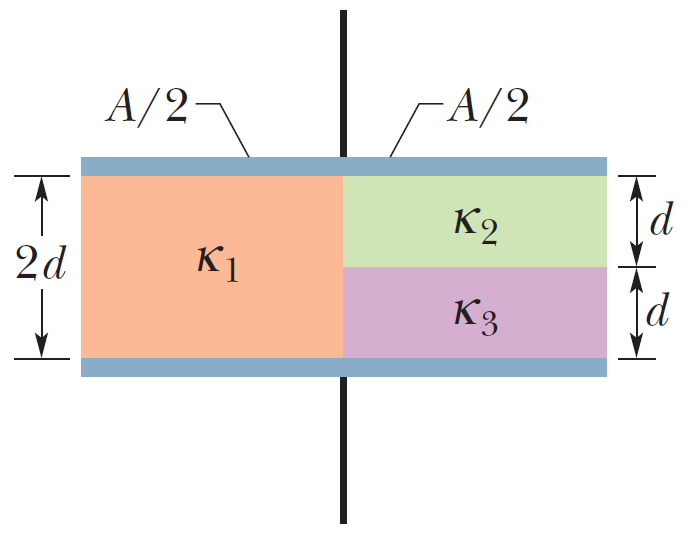
\includegraphics[height=0.3\textheight, width=0.75\textwidth,keepaspectratio]{images/capacitor1.png}
\end{center}

\mk{15} \yr{PHY 129 | L-1/T-1 | 2022-23}

\item What happens to the electric field intensity in a capacitor when a dielectric material is inserted? Draw the capacitor with and without dielectric and clarify your answer in terms of molecular theory.
\mk{20} \yr{PHY 109 | L-1/T-1 | Jan 2020}

\item A $20\mu F$ air-insulated parallel plate capacitor is charged to $300$~V. The capacitor is then disconnected from the battery, and its plate separation is doubled. Find the stored energy (i) before and (ii) after the plate separation increases. Where does the extra energy come from?
\mk{20} \yr{PHY 109 | L-1/T-1 | Jan 2020}

\item What is a capacitor? Define the capacitance of a capacitor. Mention some applications of capacitors.
\mk{12} \yr{PHY 109 | L-1/T-1 | 2016-17}

\item Derive an expression for the capacitance of a spherical capacitor with inner radius $a$ and outer radius $b$.
\mk{18} \yr{PHY 109 | L-1/T-1 | 2016-17}

\item A parallel plate capacitor of plate area $A$ and plate separation $d$ is filled with two dielectric materials such that half the plate area has dielectric constant $k_1$ and the other half has $k_2$. Calculate the capacitance.
\mk{16.5} \yr{PHY 109 | L-1/T-1 | 2016-17}

\end{enumerate}


\label{sec:s26}
\subtopic{cA}{S2.6 \quad Magnetic Field \& Forces}

\begin{enumerate}  

\item In an experiment designed to measure the magnitude of a uniform magnetic field, electrons are accelerated from rest through a potential difference of $350\text{ V}$. The electrons travel along a circular path because of the magnetic force exerted on them, and the radius of the path is measured to be $7.5\text{ cm}$. The magnetic field is perpendicular to the beam, what is the magnitude of the magnetic field?
  \mk{8} \yr{PHY 129 | L-1/T-1 | 2024-25}

\item Consider a rectangular loop of wire carrying a current and free to rotate about a fixed axis, placed in a magnetic field. Describe the mechanism and show that the total torque on the coil has magnitude $\tau = (NiA)B\sin\theta$, where the terms have their usual meaning.
\begin{center}
  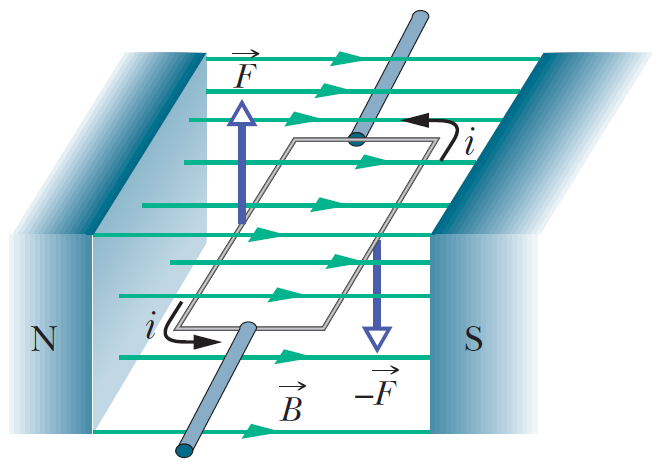
\includegraphics[height=0.2\textheight, width=0.75\textwidth,keepaspectratio]{images/torque.png}
\end{center}
\mk{11} \yr{PHY 129 | L-1/T-1 | 2023-24}


\item Why do two wires with current flowing in the same direction attract each other, and two wires with current flowing in opposite directions repel? Explain using appropriate figures.
\mk{20} \yr{PHY 109 | L-1/T-1 | Jan 2020}

\item Two long parallel wires carry currents $i_1$ and $i_2$ in opposite directions. What are the magnitude and direction of the net magnetic field at point $P$? Given $i_1 = 10$~A, $i_2 = 30$~A and $d = 5.5$~cm.


\begin{center}

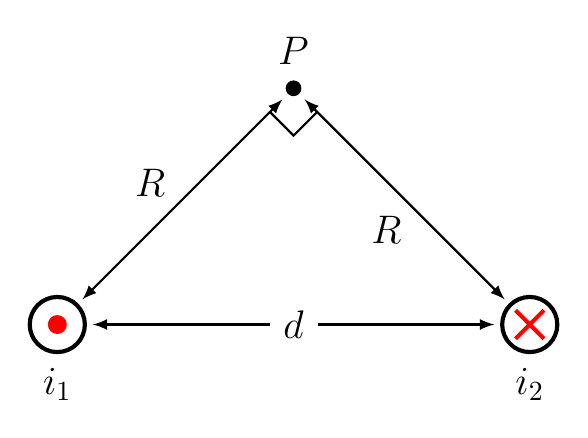
\begin{tikzpicture}[
    >={latex},
    thick,
    font=\Large
]

    % Define standard coordinates
    \coordinate (I1) at (-3, 0);
    \coordinate (I2) at (3, 0);
    \coordinate (P)  at (0, 3);
    
    % Vectors R (Drawn first so they lie beneath the right-angle marker)
    \draw[<->, shorten <=0.45cm, shorten >=0.2cm] (I1) -- (P) node[midway, above left] {$R$};
    \draw[<->, shorten <=0.45cm, shorten >=0.2cm] (I2) -- (P) node[midway, below left] {$R$};

    % Right angle marker at P
    \draw (-0.3, 2.7) -- (0, 2.4) -- (0.3, 2.7);

    % Central Point P
    \fill (P) circle (0.1) node[above=5pt] {$P$};

    % Distance d
    \draw[<->, shorten <=0.45cm, shorten >=0.45cm] (I1) -- (I2) node[midway, fill=white, inner sep=5pt] {$d$};

    % Current i1 (Left wire - Current coming out of page)
    \draw[line width=1.5pt] (I1) circle (0.35);
    \fill[red] (I1) circle (0.12);
    \node[below=12pt] at (I1) {$i_1$};

    % Current i2 (Right wire - Current going into page)
    \draw[line width=1.5pt] (I2) circle (0.35);
    \draw[line width=1.5pt, red] (I2)++(-0.18,-0.18) -- ++(0.36,0.36);
    \draw[line width=1.5pt, red] (I2)++(-0.18,0.18) -- ++(0.36,-0.36);
    \node[below=12pt] at (I2) {$i_2$};

\end{tikzpicture}
\end{center}

\mk{20} \yr{PHY 109 | L-1/T-1 | Jan 2020}

\item A cube of edge $a$ carries a point charge $q$ at each corner. (i) Show that the magnitude of the resultant electric force on any one charge is $F = 0.2261\,q^2/\varepsilon_0 a^2$. (ii) What is the direction of $F$ relative to the cube edge?
\mk{17.5} \yr{PHY 109 | L-1/T-1 | 2016-17}

\end{enumerate}


\label{sec:s27}
\subtopic{cA}{S2.7 \quad Hall Effect}

\begin{enumerate}

\item Write a short note on the Hall effect.
\mk{part} \yr{PHY 129 | L-1/T-1 | 2022-23}

\end{enumerate}


\label{sec:s28}
\subtopic{cA}{S2.8 \quad Biot-Savart \& Amp\`ere's Laws}

\begin{enumerate}

\item Two parallel wire carrying current $i_a$ and $i_b$ in the same direction, the distance between two wires is $d$. Calculate force between the wires.
 \mk{7} \yr{PHY 129 | L-1/T-1 | 2024-25}
   
\item State the Biot-Savart law. Consider a thin, straight wire carrying a constant current $i$ and placed along the $x$ axis as shown in Figure 8(c). Show that the magnitude of the magnetic field at point $P$ due to this current can be given by $B = \frac{\mu_0 i}{4\pi a}(\cos\theta_1 - \cos\theta_2)$. \\
    What will be the value of $B$ if the wire is infinite long.
\begin{center}
  \begin{tikzpicture}[scale=1.5, >=stealth]
    % Coordinates
    \coordinate (P) at (0,3);
    \coordinate (LeftEnd) at (-2,0);
    \coordinate (RightEnd) at (2,0);
    \coordinate (Center) at (0,0);
    
    % Perpendicular line (a)
    \draw[dash pattern=on 4pt off 3pt, thick] (Center) -- (P) node[midway, right] {$a$};
    \fill (P) circle (1.5pt) node[above] {$P$};
    
    % Main current-carrying wire at the bottom
    \draw[thick] (-2.5,0) -- (2.5,0);
        \draw[thick] (-2.5,-0.1) -- (2.5,-0.1);

    
    % Current direction arrow and label 'i'
    \draw[->, ultra thick] (-2.3,-0.3) -- (-1.5,-0.3) node[midway, below] {$i$};
    
    % Dashed lines from P to wire ends
    \draw[dash pattern=on 4pt off 3pt] (P) -- (LeftEnd);
    \draw[dash pattern=on 4pt off 3pt] (P) -- (RightEnd);
    
    % --- Angle \theta_1 ---
    % Base line segment extension for clarity
    \draw (-2.5,0) -- (-2,0);
    % Arc for \theta_1
    \draw[thick] (-1.6,0) arc (0:56.3:0.4);
    \node at (-1.4,0.3) {$\theta_1$};
    
    % --- Angle \theta_2 ---
    % Arc for \theta_2
    \draw[thick] (2.4,0) arc (0:123.7:0.4);
    \node at (2.2,0.5) {$\theta_2$};
    
    % --- Interior Angle labels near P ---
    % Angle on left side of perpendicular: 90^\circ - \theta_1
    \draw (0,2.5) arc (-90:-123.7:0.5);

    
    % Angle on right side of perpendicular: 90^\circ + \theta_2 (or supplementary tracking)
    \draw (0,2.4) arc (-90:-56.3:0.6);

    
\end{tikzpicture}
\end{center}
 \mk{12} \yr{PHY 129 | L-1/T-1 | 2024-25}


\item State and explain Biot-Savart law and Faraday's law with suitable figures.
\mk{8} \yr{PHY 129 | L-1/T-1 | 2023-24}

\item Describe how the Lorentz force on a metal wire can affect the motion of a charged particle. By drawing the appropriate schematic diagrams of the apparatus, explain how J.~J.~Thomson came to the discovery of the electron.
\mk{25} \yr{PHY 129 | L-1/T-1 | 2022-23}

\item Point $P$ is at perpendicular distance $R = 25.1$~cm from one end of a straight wire of length $L = 13.6$~cm carrying current $i = 0.693$~A (note that the wire is not long). What is the magnitude of the magnetic field at $P$?
\begin{center}
  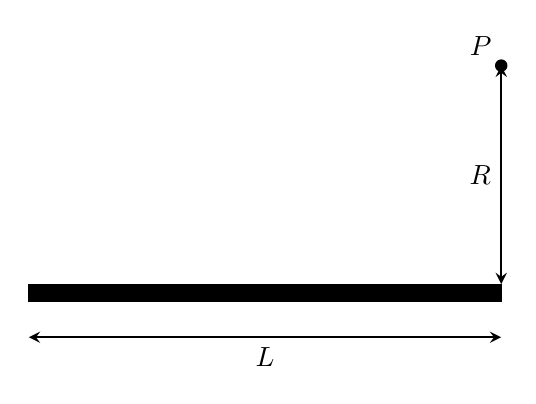
\begin{tikzpicture}[scale=1.5, >=stealth]
    % --- Thick Bar/Rod at the bottom ---
    % Drawing a rectangular bar to match the thick solid rod in the image
    \filldraw[fill=black, draw=black] (0,0) rectangle (4,0.15);
    
    % --- Point P and Vertical Distance R ---
    % Vertical arrowed line from the right end of the bar
    \draw[<->, thick] (4,0.15) -- (4,2.0) node[midway, left] {$R$};
    
    % Point P at the top of the vertical line
    \fill (4,2.0) circle (1.5pt) node[above left] {$P$};
    
    % --- Horizontal Dimension L ---
    % Shifted slightly downward from the bar for clean spacing
    \draw[<->, thick] (0,-0.3) -- (4,-0.3) node[midway, below] {$L$};
    
\end{tikzpicture}
\end{center}

\mk{part} \yr{PHY 129 | L-1/T-1 | 2022-23}

\item State and explain (i) Biot-Savart law and (ii) Ampere's law. Briefly describe the pros and cons of each of these laws.
\mk{12} \yr{PHY 129 | L-1/T-1 | 2021-22}
\variant{PHY 109 | 2017-18; PHY 109 | 2018-19}

\item A cylindrical conducting wire of radius $R$ carries current $I$ distributed uniformly across the cross-section. Using Ampere's law, calculate the magnetic induction $B$ at a distance $r$ from the centre for (i) outside ($r>R$), (ii) inside ($r<R$), and (iii) surface ($r=R$). Draw schematically $B(r)$ as a function of $r$.
\mk{22.5} \yr{PHY 109 | L-1/T-1 | 2018-19}

\item A long coaxial cable consists of an inner solid conductor of radius $a$ and an outer hollow conductor with inner radius $b$ and outer radius $c$, carrying equal and opposite currents $I$. Find the magnetic induction $B$ at (i) $r$ within the inner conductor ($r < a$) and (ii) between the two conductors ($a < r < b$).
\mk{12} \yr{PHY 109 | L-1/T-1 | 2018-19}



\end{enumerate}

\label{sec:s29}
\subtopic{cA}{S2.9 \quad Electromagnetic Induction \& Inductance}

\begin{enumerate}

\item For an RL circuit in which the current is rising, find out the current through the inductor as a function of time. Hence explain the idea of the inductive time constant.
\mk{13} \yr{PHY 129 | L-1/T-1 | 2021-22}
\variant{PHY 109 | 2020-21}

\item State and explain Faraday's law and Lenz's law for electromagnetic induction.
\mk{12} \yr{PHY 109 | L-1/T-1 | 2020-21}

\item A circuit contains an inductance $L$ and a resistance $R$ in series with a battery of emf $\varepsilon$. Obtain expressions for the growth and decay of current in the circuit. What is the inductive time constant?
\mk{22.5} \yr{PHY 109 | L-1/T-1 | 2020-21}

\item The time constant of an inductance coil is $2.2$~ms. If a resistance of $90\ \Omega$ is added in series, the time constant reduces to $0.75$~ms. Find the inductance and resistance of the coil.
\mk{12} \yr{PHY 109 | L-1/T-1 | 2020-21}

\item Briefly explain the term self-inductance and hence derive expressions for self-inductances for toroids having circular and rectangular cross-sections.
\mk{20.5} \yr{PHY 109 | L-1/T-1 | 2017-18}

\item A rectangular loop of $N$ turns with length $a$ and width $b$ is rotated at frequency $v$ in a uniform magnetic field of induction $B$. (i) Show that an induced emf $E = 2\pi v N ab B\sin(2\pi v t) = E_0\sin(2\pi v t)$ appears in the loop. (ii) Design a loop that will produce an emf with $E_0 = 220$~V when rotated at $50$~rev/s in a field of $5000$~Gauss.
\mk{8} \yr{PHY 109 | L-1/T-1 | 2017-18}

\item State and explain Faraday's law of electromagnetic induction. A conducting bar moves along two parallel conducting rails with constant velocity $v$ in the presence of a uniform magnetic field $B$ into the plane. What emf is induced in the bar?
\mk{15.5} \yr{PHY 109 | L-1/T-1 | 2015-16}

\item What is inductance? Derive expressions for inductance of a long solenoid and a toroid having circular cross-section.
\mk{24} \yr{PHY 109 | L-1/T-1 | 2015-16}

\item Suppose two inductors with equal inductance $L$ are connected in parallel, separated by a large distance. Calculate the equivalent inductance.
\mk{7.5} \yr{PHY 109 | L-1/T-1 | 2015-16}

\end{enumerate}

\label{sec:s210}
\subtopic{cA}{S2.10 \quad Solenoid and Toroid}

\begin{enumerate}
  \item A long solenoid has $n = 400\text{ turns per meter}$ and carries a current given by $I = (30.0\text{ A})(1 - e^{-1.60t})$ as shown in Figure. Inside the solenoid and coaxial with it is a coil that has a radius of $6.00\text{ cm}$ and consists of a total of $N = 250\text{ turns}$ of fine wire. What emf is induced in the coil by the changing after $t = 2.0\text{ sec}$?
\begin{center}
  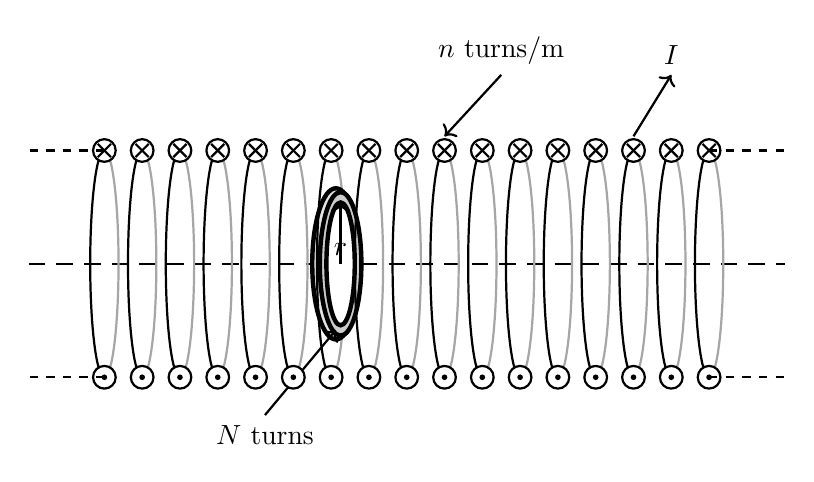
\begin{tikzpicture}[scale=1.2]
    % --- Central Axis Line ---
    \draw[thick, dash pattern=on 6pt off 4pt] (-4,0) -- (4,0);

    % --- Background Solenoid Lines (Back half of the loops) ---
    \foreach \x in {-3.2,-2.8,...,3.2} {
        \draw[thick, gray!70] (\x,-1.2) arc (-90:90:0.15 and 1.2);
    }

    % --- Coaxial Inner Coil (N turns) ---
    \draw[ultra thick, fill=gray!20] (-0.75,0) ellipse (0.25 and 0.8);
    \draw[ultra thick, fill=gray!40] (-0.70,0) ellipse (0.22 and 0.76);
    \draw[ultra thick, fill=white] (-0.70,0) ellipse (0.15 and 0.65);
    
    % Radius indicator 'r'
    \draw[thick, ->] (-0.70,0) -- (-0.70,0.65) node[midway, below] {$r$};
    
    % Label for N turns
    \draw[thick, <-] (-0.75,-0.7) -- (-1.5,-1.6) node[below] {$N \text{ turns}$};

    % --- Foreground Solenoid Lines (Front half of the loops) ---
    \foreach \x in {-3.2,-2.8,...,3.2} {
        \draw[thick] (\x,1.2) arc (90:270:0.15 and 1.2);
    }

    % --- Top and Bottom Solenoid Cross Sections (Interchanged) ---
    \foreach \x in {-3.2,-2.8,...,3.2} {
        % --- Top Turns: CROSSES (\otimes effect) ---
        \filldraw[fill=white, draw=black, thick] (\x,1.2) circle (0.12);
        % Drawing the 'X' inside the top circle
        \draw[thick] (\x-0.07,1.2-0.07) -- (\x+0.07,1.2+0.07);
        \draw[thick] (\x-0.07,1.2+0.07) -- (\x+0.07,1.2-0.07);
        
        % --- Bottom Turns: DOTS (\odot effect) ---
        \filldraw[fill=white, draw=black, thick] (\x,-1.2) circle (0.12);
        \fill[black] (\x,-1.2) circle (0.03); % Center dot
    }

    % --- Solenoid Outer Boundaries (Dashed extensions) ---
    \draw[thick, dashed] (-3.2,1.2) -- (-4,1.2);
    \draw[thick, dashed] (3.2,1.2) -- (4,1.2);
    \draw[thick, dashed] (-3.2,-1.2) -- (-4,-1.2);
    \draw[thick, dashed] (3.2,-1.2) -- (4,-1.2);

    % --- Labels and Arrows ---
    % n turns/m label
    \draw[thick, <-] (0.4, 1.35) -- (1.0, 2.0) node[above] {$n \text{ turns/m}$};
    
    % Current I label
    \draw[thick, ->] (2.4, 1.35) -- (2.8, 2.0) node[above] {$I$};

\end{tikzpicture}

\end{center}

  \mk{8} \yr{PHY 129 | L-1/T-1 | 2024-25}

\item What are solenoid and toroid? Derive expression of $B$ for solenoid and toroid.
\mk{18} \yr{PHY 109 | L-1/T-1 | 2017-18}

\end{enumerate}


\label{sec:s211}
\subtopic{cA}{S2.11 \quad RC, LR, LC \& LRC Circuits}

\begin{enumerate}

\item Explain why the LC circuit is known as an electromagnetically oscillatory circuit. Derive the differential equation describing the oscillations of a resistanceless LC circuit and show that the angular frequency is $\omega = 1/\sqrt{LC}$.
\mk{17} \yr{PHY 129 | L-1/T-1 | 2023-24}

\item A $2.37$~mF capacitor is charged to $55$~V and then connected in series with a $15$~mH coil at $t = 0$ to form an LC oscillator. (i) What is the potential difference $V_L(t)$ across the inductor as a function of time? (ii) What is the maximum rate $di/dt$ at which the current changes in the circuit?
\mk{10} \yr{PHY 129 | L-1/T-1 | 2023-24}

\item Deduce the frequency and quality factor for a circuit with $L = 2$~mH, $C = 5$~pF and $R = 0.2$~$\Omega$.
\mk{10} \yr{PHY 109 | L-1/T-1 | 2008-09}

\end{enumerate}

\label{sec:s212}
\subtopic{cA}{S2.12 \quad Mass Spectrometer}

\begin{enumerate}

\item An ion of mass $m$ and charge $q$ is accelerated from rest by a potential difference $V$ and enters a uniform magnetic field $B$ perpendicular to its path. Given $B = 80$~mT, $V = 1000$~V, $q = +1.6022\times10^{-19}$~C, and the ions strike the detector at $x = 1.6254$~m, find the mass $m$ of the individual ions.
\mk{10} \yr{PHY 129 | L-1/T-1 | 2021-22}

\begin{center}
  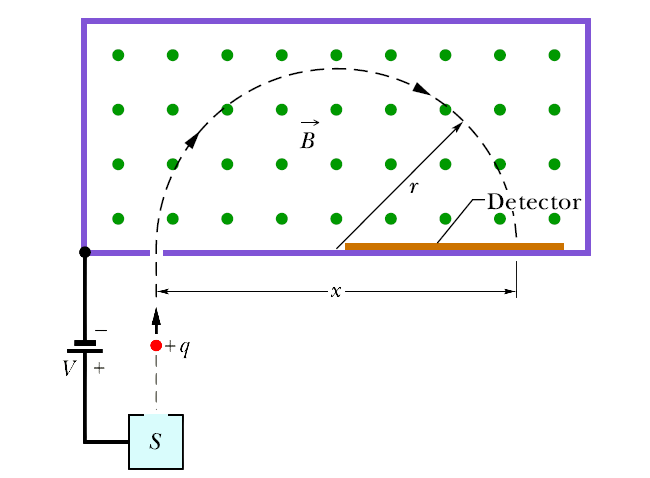
\includegraphics[height=0.3\textheight, width=0.75\textwidth,keepaspectratio]{images/massSpectrometer.png}
\end{center}

\end{enumerate}

\label{sec:s213}
\subtopic{cA}{S2.13 \quad Magnetic Materials \& Computing Applications}

\begin{enumerate}

\item Briefly mention the properties of diamagnetic, paramagnetic, ferromagnetic and antiferromagnetic materials with examples. Sketch magnetic moment orientations and $M$--$H$ response.
\mk{10} \yr{PHY 129 | L-1/T-1 | 2023-24}

\end{enumerate}

%% ══════════════════════════════════════════════════════════════════════
%%  PART III: WAVE MECHANICS
%% ══════════════════════════════════════════════════════════════════════
\secdivider{Part III}{Wave Mechanics}%
  {Quantum Theory, Schr\"odinger Equation, Particle in a Box}%
  {Failure of classical mechanics $\cdot$ Wave-particle duality $\cdot$ Uncertainty principle $\cdot$ Postulates of QM $\cdot$ Wave function $\cdot$ Operators $\cdot$ Schr\"odinger equation $\cdot$ Expectation value $\cdot$ Ehrenfest theorem $\cdot$ Eigenfunction \& eigenvalues $\cdot$ Particle in a box $\cdot$ Square well potential $\cdot$ Linear harmonic oscillator}%
  {cC}{green}

\markboth{Part III: Wave Mechanics}{Part III: Wave Mechanics}
\label{sec:S3}
\section*{Part III \quad Wave Mechanics}
\addcontentsline{toc}{section}{Part III: Wave Mechanics}

\label{sec:s31}
\subtopic{cA}{S3.1 \quad Failure of Classical Mechanics \& Historical Origins}

\begin{enumerate}

\item Based on Planck's constant, briefly explain when a classical description is sufficient and when a quantum description is necessary.
\mk{8} \yr{PHY 129 | L-1/T-1 | 2023-24}

\item Describe the experimental facts of blackbody radiation briefly. Why can this phenomenon not be explained in terms of classical physics?
\mk{12} \yr{PHY 129 | L-1/T-1 | 2021-22}

\item Briefly explain the inadequacy of classical mechanics for which quantum mechanics is introduced.
\mk{10} \yr{PHY 109 | L-1/T-1 | 2018-19}

\item Write down the differences between classical and quantum mechanics.
\mk{8} \yr{PHY 109 | L-1/T-1 | 2016-17}

\end{enumerate}

\label{sec:s32}
\subtopic{cA}{S3.2 \quad Wave-Particle Duality}

\begin{enumerate}

\item What are matter waves in the context of quantum mechanics? Discuss the propagation speed of a de Broglie wave associated with a moving particle.
\mk{10} \yr{PHY 129 | L-1/T-1 | 2024-25}

\item Define phase velocity and group velocity for de Broglie waves. Derive expressions for both in terms of the particle's energy and momentum.
\mk{15} \yr{PHY 129 | L-1/T-1 | 2024-25}

\item An electron exhibits a de Broglie wavelength of $\lambda = 2.10\text{ pm}$. Calculate: its
\begin{enumerate}
        \item[(i)] kinetic energy,
        \item[(ii)] phase velocity, and
        \item[(iii)] group velocity.
\end{enumerate}  
\mk{10} \yr{PHY 129 | L-1/T-1 | 2024-25}

\item Calculate the de Broglie wavelengths for (i) an electron of kinetic energy $72$~MeV and (ii) a $710$~g bullet moving at $920$~m/s.
\mk{part} \yr{PHY 129 | L-1/T-1 | 2023-24}

\end{enumerate}

\label{sec:s33}
\subtopic{cA}{S3.3 \quad Uncertainty Principle}

\begin{enumerate}

\item State and explain the uncertainty principle. Write down three uncertainty relations.
\mk{7} \yr{PHY 129 | L-1/T-1 | 2024-25}

\item Derive the uncertainty relation relation using wave and particle approaches.
\mk{18} \yr{PHY 129 | L-1/T-1 | 2024-25}

\item An excited atom gives up its excess energy by emitting a photon of characteristic frequency. The average period that elapes between the  excitation of an atom and the time it radiates $1.2\times 10^{-8}s$. Find the inherent uncertainty in the frequency of the photon.
\mk{10} \yr{PHY 129 | L-1/T-1 | 2024-25}


\item State Heisenberg's uncertainty principle. In case of two matter-waves that superimpose, show that $\Delta x \cdot \Delta p \geq \hbar/2$.
\mk{24.5} \yr{PHY 109 | L-1/T-1 | 2020-21}

\end{enumerate}


\label{sec:s34}
\subtopic{cA}{S3.4 \quad Postulates of QM \& Wave Function}

\begin{enumerate}

\item Obtain the time-dependent Schrödinger equation by considering that the wave function $\Psi$ corresponds to the wave variable $y$ of wave motion in general.
\mk{20} \yr{PHY 129 | L-1/T-1 | 2023-24}

\item Write down the required characteristics of the wave function. Distinguish between the wave function and the probability density function.
\mk{10} \yr{PHY 129 | L-1/T-1 | 2022-23}
\variant{PHY 109 | 2016-17}

\item How is the energy eigenfunction of an electron strongly bound to its atomic nucleus different from that of a free electron? Draw a schematic representation of the allowed energy levels of a bound electron in an infinite square potential well.
\mk{15} \yr{PHY 129 | L-1/T-1 | 2022-23}
\variant{PHY 129 | 2021-22}

\item ``Schrödinger equation cannot be derived from other basic principles of physics; it is a basic principle in itself'' --- justify this statement.
\mk{13} \yr{PHY 129 | L-1/T-1 | 2021-22}
\variant{PHY 129 | 2023-24}

\item Draw schematically the wave function $\psi$ and the probability function $\psi^*\psi$ for an electron in an infinite square well potential for different $n$-values. What conclusions can be drawn for the probability of finding electrons in $n = 1$, $2$, and $100$ states?
\mk{10} \yr{PHY 129 | L-1/T-1 | 2021-22}

\item Write down the properties of wave functions. A wave function is defined as
\[
  \Psi(x,0) = \begin{cases} 3x^2 + 5 & -6 < x < 3 \\ -2x + 3 & 3 \leq x < 7 \\ 0 & \text{otherwise} \end{cases}
\]
(i) Normalize the wave function. (ii) Plot $\Psi(x,0)$ as a function of $x$. (iii) What is the probability of finding the particle to the right of $x = 0$?
\mk{40} \yr{PHY 109 | L-1/T-1 | Jan 2020}

\item How is the time-dependent Schr\"odinger equation different from the time-independent form?
\mk{8} \yr{PHY 109 | L-1/T-1 | Jan 2020}

\item Consider the wave function $\Psi(x,t) = Ae^{-\lambda|x|}e^{-i\omega t}$ where $A$, $\lambda$, and $\omega$ are positive real constants. (i) Normalize $\Psi$. (ii) Determine the expectation values of $x$ and $x^2$.
\mk{14} \yr{PHY 109 | L-1/T-1 | 2016-17}

\item What do you mean by normalization? Briefly discuss the physical significance of normalization of a wave function.
\mk{7.5} \yr{PHY 109 | L-1/T-1 | 2015-16}

\item Show that if a wave function is normalized at $t = 0$, then it is normalized for any time $t$.
\mk{20} \yr{PHY 109 | L-1/T-1 | 2015-16}

\item At time $t = 0$, a wave function is represented by
\[
  \Psi(x,0) = \begin{cases} A\frac{x}{a} & 0 < x < a \\ A\frac{b-x}{b-a} & a \leq x \leq b \\ 0 & \text{otherwise} \end{cases}
\]
where $A$, $a$, and $b$ are constants. (i) Normalize $\Psi(x,0)$. (ii) Sketch $\Psi(x,0)$ as a function of position.
\mk{19} \yr{PHY 109 | L-1/T-1 | 2015-16}

\end{enumerate}

\label{sec:s35}
\subtopic{cA}{S3.5 \quad Operators \& Schr\"odinger Equation}

\begin{enumerate}

\item State and explain the Hamiltonian operator of a quantum particle. Write down the Schr\"odinger equation using the Hamiltonian operator.
\mk{8} \yr{PHY 129 | L-1/T-1 | 2023-24}

\item What is a ``Quantum Mechanical Operator''? Write down the expressions for the momentum operator and energy operator.
\mk{10} \yr{PHY 129 | L-1/T-1 | 2022-23}
\variant{PHY 129 | 2021-22; PHY 129 | 2023-24}

\item What is an operator? Write down the required expressions for momentum, energy and Hamiltonian operators.
\mk{12} \yr{PHY 129 | L-1/T-1 | 2021-22}

\item How is the energy eigenfunction of an electron strongly bound to its atomic nucleus different from that of a free electron?
\mk{13} \yr{PHY 129 | L-1/T-1 | 2021-22}

\item Draw schematically the potential well and energy levels of (i) a hydrogen atom, (ii) a particle in a box, and (iii) a harmonic oscillator.
\mk{10} \yr{PHY 129 | L-1/T-1 | 2021-22}

\item Consider a particle is moving in one dimension whose wavefunction can be expressed by,
\[
\Psi(x,t) = A e^{i(kx - \omega t)}
\]
where, $A$ is a constant quantity. If $k$ and $\omega$ denote corresponding wave number and angular frequency, then obtain

\begin{enumerate}
    \item[(i)] Quantum mechanical linear momentum operator ($\hat{p}$)
    \item[(ii)] Quantum mechanical angular momentum operators ($\hat{l}_x, \hat{l}_y, \hat{l}_z$)
\end{enumerate}

\noindent In the steady state condition, obtain time independent Schrödinger equation.
\mk{24.67} \yr{PHY 109 | L-1/T-1 | 2020-21}



\item Using commutation relations on wave function $\psi$, show that 
\begin{align*}
    \text{(i)} \quad & [\hat{l}_x, \hat{y}] = i \hbar \hat{z} \\
    \text{(ii)} \quad & [\hat{z}, \hat{p}_y] = 0
\end{align*}
\mk{12} \yr{PHY 109 | L-1/T-1 | 2020-21}

\item Derive the one-dimensional (i) time-dependent and (ii) time-independent Schr\"odinger equation of a bound particle.
\mk{26.5} \yr{PHY 109 | L-1/T-1 | 2018-19}
\variant{PHY 109 | 2015-16}

\item What is Hermitian operator? Show that the eigenvalues of a Hermitian operator are real.
\mk{10} \yr{PHY 109 | L-1/T-1 | 2018-19}
\variant{PHY 109 | 2020-21}

\item Derive the time-independent Schr\"odinger equation for a particle moving in a potential. Write down the physical significance of the wave function.
\mk{15} \yr{PHY 109 | L-1/T-1 | 2017-18}

\item Define the Hamilton operator. Show that the momentum operator commutes with the free particle Hamilton operator, i.e. $[\hat{H}, \hat{p}] = 0$.
\mk{part} \yr{PHY 109 | L-1/T-1 | 2017-18}

\item Solve the time-independent Schr\"odinger equation to derive an expression for the wave function when a particle of mass $m$ is confined inside an infinite square well of width $a$.
\mk{24.5} \yr{PHY 109 | L-1/T-1 | 2016-17}

\item Show that there is no acceptable solution to the time-independent Schr\"odinger equation for the infinite square well with negative energy.
\mk{14} \yr{PHY 109 | L-1/T-1 | 2016-17}

\item Derive the time-independent Schr\"odinger equation from the time-dependent Schr\"odinger equation for a stationary state.
\mk{17} \yr{PHY 109 | L-1/T-1 | 2015-16}

\end{enumerate}

\label{sec:s36}
\subtopic{cA}{S3.6 \quad Expectation Value \& Ehrenfest Theorem}

\begin{enumerate}

\item State and explain Ehrenfest's theorem. How can this theorem be connected to the Hamilton-Jacobi equations of classical mechanics? Consider a charged oscillator of positive charge $q$ and mass $m$ subjected to an oscillating electric field $E_0\cos\omega t$ with Hamiltonian $H = \frac{p^2}{2m} + \frac{k}{2}x^2 + qE_0 x\cos\omega t$. Calculate $\frac{d\langle x\rangle}{dt}$, $\frac{d\langle p\rangle}{dt}$, $\frac{d\langle H\rangle}{dt}$. Solve the equation for $\frac{d\langle p\rangle}{dt}$ and obtain $\langle x\rangle(t)$ such that $\langle x\rangle(0) = X_0$.
\mk{17} \yr{PHY 129 | L-1/T-1 | 2023-24}

\item Calculate the expectation values of position and kinetic energy for the 4th excited state of a particle inside an infinite square well.
\mk{32} \yr{PHY 109 | L-1/T-1 | Jan 2020}

\item State and prove Ehrenfest's theorem. Write down the physical significance of Ehrenfest's theorem.
\mk{24.5} \yr{PHY 109 | L-1/T-1 | 2016-17}
\variant{PHY 129 | 2023-24}

\end{enumerate}

\label{sec:s37}
\subtopic{cA}{S3.7 \quad Eigenfunction \& Eigenvalues}

\begin{enumerate}

\item What is Hermitian operator? Show that the eigenvalues of a Hermitian operator are real.
\mk{10} \yr{PHY 109 | L-1/T-1 | 2018-19}
\variant{PHY 109 | 2020-21}

\end{enumerate}

\label{sec:s38}
\subtopic{cA}{S3.8 \quad Particle in a Box}

\begin{enumerate}

\item Derive the infinite square well energy quantization law directly from the de Broglie relation by fitting an integral number of half de Broglie wavelengths into the width $a$ of the well.
\mk{12} \yr{PHY 129 | L-1/T-1 | 2021-22}

\item Consider a particle of mass $m$ bouncing back and forth inside a box along the $x$ direction with insurmountable walls at $x = 0$ and $x = L$. (i) Obtain the expression for energy. (ii) Obtain the normalized wave function. (iii) Show that the expectation value of the linear momentum is zero.
\mk{22} \yr{PHY 109 | L-1/T-1 | 2020-21}

\item Briefly write down the statements of Kepler's laws of planetary motion and hence show that the angular momentum $L$ is conserved.
\mk{12} \yr{PHY 109 | L-1/T-1 | 2018-19}

\item Consider that an electron is placed in a box $1.2$~\AA\ wide while a $10$~g marble is placed in a box $10$~cm wide. Compute the permitted energy levels in both cases and explain why we do not experience energy quantization.
\mk{12} \yr{PHY 109 | L-1/T-1 | 2018-19}

\item Consider a particle moving freely in a one-dimensional box of length $L$ with $V(x) = 0$ for $0 < x < L$ and $V = \infty$ otherwise. (i) Find out the energy. (ii) Find the normalized wave function.
\mk{21.5} \yr{PHY 109 | L-1/T-1 | 2017-18}
\variant{PHY 109 | 2016-17; PHY 109 | 2018-19; PHY 109 | 2020-21}

\end{enumerate}

\label{sec:s39}
\subtopic{cA}{S3.9 \quad Square Well Potential}

\begin{enumerate}

\item A potential well of height $U$ and width $L$ with square corners contains a particle whose energy $E$ is less than $U$. (i) Find out the wave functions of the particle. (ii) Illustrate the wave functions and probability densities of the particle. (iii) Interpret the tunneling effect of the particle.
\mk{11} \yr{PHY 129 | L-1/T-1 | 2023-24}

\item Protons with energies of $1.2$~eV and $2.2$~eV are incident on a barrier of height $12.0$~eV and width $0.60$~nm. (i) Find their respective transmission probabilities. (ii) How are these affected if the barrier is doubled in width?
\mk{10} \yr{PHY 129 | L-1/T-1 | 2023-24}
\variant{PHY 129 | 2022-23}

\item Explain the quantum mechanical tunneling effect and its significant applications. Illustrate the wave-particle duality of the electron using a schematic diagram of the quantum mechanical tunneling effect.
\mk{15} \yr{PHY 129 | L-1/T-1 | 2022-23}

\item Electrons with energies of $1.0$~eV and $2.0$~eV are incident on a barrier $10.0$~eV high and $0.50$~nm wide. (i) Find their respective transmission probabilities. (ii) How are these affected if the barrier is doubled in width?
\mk{10} \yr{PHY 129 | L-1/T-1 | 2022-23}

\item Explain briefly the quantum mechanical tunneling effect. On which factor does the tunneling effect critically depend? Write down some engineering applications of the tunneling effect.
\mk{13} \yr{PHY 129 | L-1/T-1 | 2021-22}
\variant{PHY 129 | 2022-23}

\item Estimate the penetration distance $\Delta x$ for a very small dust particle of radius $10^{-6}$~m, density $10^4$~kg/m$^3$, velocity $10^{-2}$~m/s, if the particle impinges on a potential step of height equal to twice its kinetic energy in the region to the left of the step.
\mk{10} \yr{PHY 129 | L-1/T-1 | 2021-22}
\variant{PHY 129 | 2022-23}

\end{enumerate}

\label{sec:s40}
\subtopic{cA}{S3.10 \quad Harmonic Oscillator}

\begin{enumerate}
    \item Distinguish between the classical and quantum harmonic oscillator.
    \mk{7} \yr{PHY 129 | L-1/T-1 | 2024-25}

    \item Find out the energy eigenvalue and wave function for harmonic oscillator. Discuss the similarities and dissimilarities of probability densities for lower and higher quantum numbers.
     \mk{18} \yr{PHY 129 | L-1/T-1 | 2024-25}

    \item Find the expectation values $\langle x \rangle$ for the first two states of a harmonic oscillator.
 \mk{10} \yr{PHY 129 | L-1/T-1 | 2024-25}

  \end{enumerate}

%% ══════════════════════════════════════════════════════════════════════
%%  PART IV: MISCELLANEOUS / NOT IN SYLLABUS
%% ══════════════════════════════════════════════════════════════════════
\secdivider{Part IV}{Miscellaneous / Not in Syllabus}%
  {Physical Optics $\cdot$ Heat \& Thermodynamics $\cdot$ Waves \& Oscillation}%
  {Included from past PHY\,109 papers for reference only --- these topics fall outside the PHY\,129 syllabus}%
  {cE}{orange}

\markboth{Part IV: Miscellaneous / Not in Syllabus}{Part IV: Miscellaneous / Not in Syllabus}
\label{sec:S4}
\section*{Part IV \quad Miscellaneous / Not in Syllabus}
\addcontentsline{toc}{section}{Part IV: Miscellaneous / Not in Syllabus}

{\small\textcolor{cE}{\textit{Note: The following questions appeared in past PHY\,109 papers but fall \textbf{outside} the PHY\,129 syllabus. Included for reference only.}}
\vspace{4pt}}

%% ── S4a ───────────────────────────────────────────────────────────────
\label{sec:s4a}
\subtopic{cA}{S4a \quad Heat \& Thermodynamics}

\begin{enumerate}

\item From the Maxwell-Boltzmann distribution $f(c) = 4\pi\left(\frac{m}{2\pi kT}\right)^{3/2}c^2 e^{-mc^2/2kT}$, obtain expressions for average velocity, rms velocity, and most probable velocity. Evaluate the ratio of these velocities.
\mk{38.5} \yr{PHY 109 | L-1/T-1 | 2020-21}

\item The mean free path of molecules of a certain gas at pressure $P$ and temperature $T$ is $2\times10^{-6}$~cm. Find the mean free path under: (i) pressure $P\times 10^{-6}$ and temperature $T$, and (ii) pressure $P/2$ and temperature $2T$.
\mk{8} \yr{PHY 109 | L-1/T-1 | 2020-21}

\item Using appropriate Maxwell's thermodynamic relations, deduce that for a van der Waals gas $C_P - C_V = R\left(1 + \frac{2a}{RTV}\right)$.
\mk{20} \yr{PHY 109 | L-1/T-1 | 2020-21}

\item The critical temperature and pressure of helium are $-263^\circ$C and $2.22$~atm. Calculate the radius of a helium atom.
\mk{30} \yr{PHY 109 | L-1/T-1 | Jan 2020}

\item The Van der Waal's equation for a gas is plotted at several temperatures as shown in Fig. 3. From the plot, answer the following questions:

\begin{enumerate}
    \item[(i)] Do any of these isotherms seemingly exhibit ideal gas behavior? If so, which one(s) and why?
    \item[(ii)] Estimate critical temperature, pressure and volume for this gas. Identify the gas from the estimated critical-point properties (Critical-point properties of different gases are given in Table 1).
    \item[(iii)] Estimate the molar volume of the liquid and vapor phases at a temperature of $273\text{ K}$ and a pressure of $4\text{ MPa}$.
\end{enumerate}

\vspace{0.8cm}
\begin{center}
  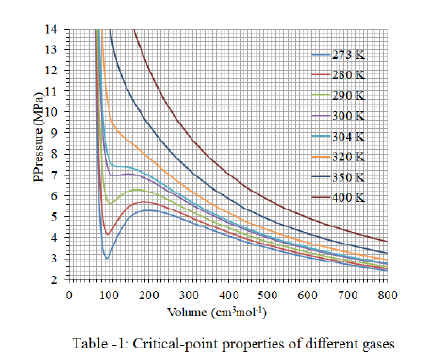
\includegraphics[height=0.35\textheight, width=0.75\textwidth,keepaspectratio]{images/critical.png}
\end{center}



\begin{tabular}{lcc}
\toprule
\textbf{Substance} & \textbf{Temperature, K} & \textbf{Pressure, MPa} \\ 
\midrule
Air & 132.5 & 3.77 \\
Ammonia & 405.5 & 11.28 \\
Argon & 151 & 4.86 \\
Benzene & 562 & 4.92 \\
Bromine & 584 & 10.34 \\
$n$-Butane & 425.2 & 3.80 \\
Carbon dioxide & 304.2 & 7.39 \\
Carbon monoxide & 133 & 3.50 \\
Carbon tetrachloride & 556.4 & 4.56 \\
Chlorine & 417 & 7.71 \\
Chloroform & 536.6 & 5.47 \\
Dichlorodifluoromethane (R-12) & 384.7 & 4.01 \\
Dichlorofluoromethane (R-21) & 451.7 & 5.17 \\
Ethane & 305.5 & 4.48 \\
Ethyl alcohol & 516 & 6.38 \\
Ethylene & 282.4 & 5.12 \\
Helium & 5.3 & 0.23 \\
\bottomrule
\end{tabular}


\item What do you mean by `degree of freedom' of a dynamical system? State the principle of equipartition of energy. Prove that for a monoatomic gas $\gamma = 5/3$, for a diatomic gas $\gamma = 7/5$, and for a triatomic gas $\gamma = 4/3$.
\mk{38.5} \yr{PHY 109 | L-1/T-1 | 2018-19}

\item Calculate the temperature at which the average translational kinetic energy of the molecules of a gas is one-third of that at $180^\circ$C.
\mk{8} \yr{PHY 109 | L-1/T-1 | 2018-19}

\item Define the term entropy and the `heat death' of the universe. Draw the temperature-entropy ($T$-$S$) diagram and prove that its area represents available energy.
\mk{25} \yr{PHY 109 | L-1/T-1 | 2018-19}

\item Derive Maxwell's expression for the mean free path: $\lambda = 1/(\sqrt{2}\pi n d^2)$ where the symbols have their usual meanings.
\mk{20} \yr{PHY 109 | L-1/T-1 | 2017-18}

\item $10$~g of water at $60^\circ$C is mixed with $30$~g of water at $20^\circ$C. Calculate the temperature of the mixture. Will the entropy of the system increase or decrease? Calculate the net change in entropy.
\mk{3} \yr{PHY 109 | L-1/T-1 | 2017-18}

\item Briefly explain conservation of linear momentum and conservation of angular momentum.
\mk{8} \yr{PHY 109 | L-1/T-1 | 2017-18}

\item (i) Define torque acting on a particle and angular momentum of a particle. (ii) Derive the relations $\tau = J\alpha$ and $L = J\omega$.
\mk{23.5} \yr{PHY 109 | L-1/T-1 | 2017-18}

\item Consider the motion of a body of mass $m$ about a massive body of mass $M$ in a circular orbit of radius $r$. Show that the total energy $E = -GMm/2r$. What is the significance of this negative energy?
\mk{15} \yr{PHY 109 | L-1/T-1 | 2017-18}

\item Calculate the number of molecules per cc of a gas if the mean free path is $3.4\times10^{-6}$~cm and the molecular diameter is $2.0\times10^{-8}$~cm. What is the collision frequency if the rms speed is $1\times10^5$~cm/s?
\mk{8} \yr{PHY 109 | L-1/T-1 | 2016-17}
\variant{PHY 109 | 2017-18}

\item Discuss the deficiencies of the perfect gas equation and obtain the van der Waals equation of state: $\left(P + \frac{a}{V^2}\right)(V - b) = RT$.
\mk{19} \yr{PHY 109 | L-1/T-1 | 2016-17}

\item Deduce expressions for critical temperature, critical pressure, and critical volume in terms of van der Waals constants. Show that $\frac{RT_c}{P_c V_c} = \frac{8}{3}$.
\mk{19.5} \yr{PHY 109 | L-1/T-1 | 2016-17}
\variant{PHY 109 | 2020-21}

\item Distinguish between isothermal and adiabatic processes. Describe the Carnot cycle. Show that the efficiency is $\eta = 1 - T_2/T_1$. Show that for a perfect gas in adiabatic transformation: (i) $PV^\gamma = \text{constant}$ and (ii) $TV^{\gamma-1} = \text{constant}$.
\mk{38.5} \yr{PHY 109 | L-1/T-1 | 2016-17}

\item Explain why the temperature of a gas drops in adiabatic expansion.
\mk{6.5} \yr{PHY 109 | L-1/T-1 | 2016-17}

\item Define the terms: (i) root mean square velocity, (ii) mean free path, (iii) degrees of freedom of a gas.
\mk{12} \yr{PHY 109 | L-1/T-1 | 2015-16}

\item Using Maxwell-Boltzmann distribution law, show that the rms velocity of molecules is $v_\text{rms} = \sqrt{3kT/m}$.
\mk{12} \yr{PHY 109 | L-1/T-1 | 2015-16}
\variant{PHY 109 | 2017-18; PHY 109 | 2020-21}

\item State the principle of equipartition of energy. Prove that for monoatomic and diatomic gases the values of $\gamma$ are $5/3$ and $7/5$ respectively.
\mk{22.5} \yr{PHY 109 | L-1/T-1 | 2015-16}
\variant{PHY 109 | 2018-19}

\item Define entropy of a substance. Show that entropy remains constant in a reversible process but increases in an irreversible process.
\mk{20.5} \yr{PHY 109 | L-1/T-1 | 2015-16}
\variant{PHY 109 | 2017-18}

\item Define and explain four fundamental thermodynamic potentials $U$, $F$, $H$ and $G$.
\mk{14} \yr{PHY 109 | L-1/T-1 | 2015-16}
\variant{PHY 109 | 2017-18; PHY 109 | 2018-19}

\item Using thermodynamic potentials, derive the Maxwell thermodynamic relations: (i) $\left(\frac{\partial S}{\partial V}\right)_T = \left(\frac{\partial P}{\partial T}\right)_V$ and (ii) $\left(\frac{\partial S}{\partial P}\right)_T = -\left(\frac{\partial V}{\partial T}\right)_P$.
\mk{12} \yr{PHY 109 | L-1/T-1 | 2015-16}
\variant{PHY 109 | 2018-19}

\item Briefly discuss Kepler's laws for planetary motions. Show that the radius vector from the sun to the planet sweeps equal areas in equal time.
\mk{29.5} \yr{PHY 109 | L-1/T-1 | 2015-16}

\item Define mean free path. Find an expression for the mean free path for gaseous molecules.
\mk{16} \yr{PHY 109 | L-1/T-1 | 2014-15}

\item Using Maxwell's distribution function, find an expression for the root-mean-square speed of gaseous molecules.
\mk{18.5} \yr{PHY 109 | L-1/T-1 | 2014-15}

\item Given that the effective diameter of an oxygen molecule is $d = 3.15\times10^{-10}$~m, calculate (i) the mean free path, (ii) the average speed, and (iii) the average collision rate for oxygen at room temperature ($27^\circ$C) and atmospheric pressure.
\mk{12} \yr{PHY 109 | L-1/T-1 | 2014-15}

\item State the second law of thermodynamics as many ways as you can. Define efficiency of a heat engine. Describe each step of the Carnot cycle and show that $\eta = 1 - T_2/T_1$.
\mk{34} \yr{PHY 109 | L-1/T-1 | 2014-15}
\variant{PHY 109 | 2012-13}

\item In a Carnot cycle, isothermal expansion takes place at $412$~K and isothermal compression at $297$~K. During the expansion, $2090$~J of heat energy are transferred to the gas. Determine (i) the work done by the gas during isothermal expansion, (ii) the heat rejected during isothermal compression, and (iii) the work done on the gas during isothermal compression.
\mk{12.5} \yr{PHY 109 | L-1/T-1 | 2014-15}

\item Prove Clausius's theorem of inequality. Using Clausius inequality show that entropy of a system always increases in an irreversible process.
\mk{24} \yr{PHY 109 | L-1/T-1 | 2013-14}

\item Calculate the change in entropy of a gas when it is heated at constant pressure.
\mk{10} \yr{PHY 109 | L-1/T-1 | 2013-14}

\item One gram-molecule of a gas expands isothermally to four times its volume. Calculate the change in entropy in terms of the gas constant.
\mk{2.5} \yr{PHY 109 | L-1/T-1 | 2013-14}

\item Deduce van der Waals equation for a real gas. Using Maxwell's thermodynamic relations, show that for a van der Waals gas $C_P - C_V = R\left(1 + \frac{2a}{RTV}\right)$ where the symbols have their usual meanings.
\mk{24} \yr{PHY 109 | L-1/T-1 | 2013-14}

\item Show that $\left(\frac{\partial T}{\partial P}\right)_S = \frac{\gamma}{\gamma-1}\left(\frac{\partial V}{\partial T}\right)_P$ where the symbols have their usual meanings.
\mk{10} \yr{PHY 109 | L-1/T-1 | 2013-14}

\item Calculate the change in melting point of ice at $0^\circ$C when the pressure is increased by $2$~atm. How much pressure is required to lower the melting point by $1^\circ$C? Given: latent heat of fusion $= 80$~cal/g, specific volumes of water and ice are $1.0001$~cc and $1.0908$~cc respectively.
\mk{12.5} \yr{PHY 109 | L-1/T-1 | 2013-14}

\item State the second law of thermodynamics in as many ways as you can.
\mk{6} \yr{PHY 109 | L-1/T-1 | 2012-13}

\item Explain the Carnot cycle with the help of a neat $P$--$V$ diagram. Show that the efficiency of a Carnot engine using an ideal gas as the working substance is $\eta = 1 - T_2/T_1$.
\mk{32} \yr{PHY 109 | L-1/T-1 | 2012-13}
\variant{PHY 109 | 2010-11}

\item An insulated vessel containing $1.8$~kg of water is placed on a hot plate. Both the water and hot plate are initially at $20^\circ$C. The temperature of the hot plate is raised very slowly to $100^\circ$C. What is the change of entropy of the water during this process?
\mk{8.5} \yr{PHY 109 | L-1/T-1 | 2012-13}

\item State and explain the principle of equipartition of energy.
\mk{15} \yr{PHY 109 | L-1/T-1 | 2012-13}
\variant{PHY 109 | 2007-08}

\item Write down Maxwell's distribution of molecular speed. Hence find the expression for root-mean-square (rms) speed.
\mk{23} \yr{PHY 109 | L-1/T-1 | 2012-13}

\item Calculate (i) the average speed and (ii) rms speed for oxygen molecules at $27^\circ$C.
\mk{8.5} \yr{PHY 109 | L-1/T-1 | 2012-13}

\item Derive van der Waals equation for a real gas. Obtain expressions for the critical volume ($V_c$), pressure ($P_c$) and temperature ($T_c$) for a real gas.
\mk{28} \yr{PHY 109 | L-1/T-1 | 2011-12}
\variant{PHY 109 | 2008-09}

\item Calculate van der Waals constants for dry air, given $T_c = 132$~K, $P_c = 37.2$~atm, and $R = 8.3$~J\,K$^{-1}$\,mol$^{-1}$.
\mk{8.5} \yr{PHY 109 | L-1/T-1 | 2011-12}

\item Explain thermodynamic functions $H$, $F$ and $G$ for a system with constant composition.
\mk{10} \yr{PHY 109 | L-1/T-1 | 2011-12}

\item Derive the Maxwell thermodynamic relation $\left(\frac{\partial S}{\partial V}\right)_T = \left(\frac{\partial P}{\partial T}\right)_V$.
\mk{28} \yr{PHY 109 | L-1/T-1 | 2011-12}
\variant{PHY 109 | 2007-08}

\item Deduce Clapeyron's latent heat equation from the Maxwell thermodynamic relations.
\mk{8.5} \yr{PHY 109 | L-1/T-1 | 2011-12}
\variant{PHY 109 | 2006-07}

\item State and explain the first law of thermodynamics. Prove that $PV^\gamma = \text{constant}$, where the symbols have their usual meanings.
\mk{34} \yr{PHY 109 | L-1/T-1 | 2010-11}

\item A quantity of dry air at $27^\circ$C is compressed (i) slowly and (ii) suddenly to $\frac{1}{3}$ of its volume. Find the change in temperature in each case. ($\gamma = 1.4$ for dry air)
\mk{12} \yr{PHY 109 | L-1/T-1 | 2010-11}

\item Describe a Carnot cycle. Obtain the expressions for the work done in each stage and the net work done in the cycle.
\mk{34} \yr{PHY 109 | L-1/T-1 | 2010-11}

\item Find the efficiency of an engine requiring $3\times10^6$~calories of heat per horse-power hour and compare it with that of a perfect reversible engine, assuming source at $1000^\circ$C and sink at $0^\circ$C. ($1\ \text{H.P.} = 746.4$~W)
\mk{12} \yr{PHY 109 | L-1/T-1 | 2010-11}

\item Evaluate the average energy of a gas molecule according to Maxwell's law of distribution of velocities.
\mk{20.5} \yr{PHY 109 | L-1/T-1 | 2008-09}

\item Derive the van der Waals equation for gases.
\mk{22.5} \yr{PHY 109 | L-1/T-1 | 2008-09}

\item Evaluate the most probable velocity of a molecule using Maxwell's law of distribution of velocities.
\mk{16} \yr{PHY 109 | L-1/T-1 | 2007-08}

\item What is the most probable velocity of a molecule of hydrogen at $27^\circ$C? Given: $k_B = 1.38\times10^{-23}$~J/K, $m = 2.34\times10^{-27}$~kg.
\mk{10} \yr{PHY 109 | L-1/T-1 | 2007-08}

\item State the law of equipartition of energy. Find general expressions for the principle of temperature measurements.
\mk{20.5} \yr{PHY 109 | L-1/T-1 | 2007-08}

\item Show that entropy remains constant in a reversible adiabatic process and increases in an irreversible process.
\mk{10} \yr{PHY 109 | L-1/T-1 | 2007-08}

\item Deduce Maxwell's thermodynamic relations.
\mk{16} \yr{PHY 109 | L-1/T-1 | 2007-08}

\item Derive Maxwell's law of distribution of velocities of gas molecules.
\mk{16} \yr{PHY 109 | L-1/T-1 | 2006-07}

\item Evaluate the most probable energy and average energy of a gas molecule according to Maxwell's law of distribution of velocities.
\mk{18} \yr{PHY 109 | L-1/T-1 | 2006-07}
\variant{PHY 109 | 2008-09}

\item Calculate the most probable velocity and energy of a hydrogen molecule at $300$~K. Given: $k_B = 1.38\times10^{-16}$~erg/K, $m = 3.34\times10^{-24}$~g.
\mk{12.5} \yr{PHY 109 | L-1/T-1 | 2006-07}

\item State and prove Carnot's theorem.
\mk{20} \yr{PHY 109 | L-1/T-1 | 2006-07}
\variant{PHY 109 | 2007-08; PHY 109 | 2008-09}

\item A Carnot engine whose source temperature is $400$~K takes $200$~cal of heat and rejects $150$~cal to the sink. Find (i)~the temperature of the sink and (ii)~the efficiency of the engine.
\mk{12.5} \yr{PHY 109 | L-1/T-1 | 2006-07}
\variant{PHY 109 | 2008-09}

\item Deduce the Clausius--Clapeyron equation for latent heat.
\mk{14} \yr{PHY 109 | L-1/T-1 | 2006-07}
\variant{PHY 109 | 2008-09}

\item What are the specific heats of an ideal gas? Show that in the limit of differential changes, the specific heat at constant volume for a monoatomic gas can be written as $C_V = \frac{1}{u}\frac{du}{dT} = \frac{3}{2}R$.
\mk{20} \yr{PHY 109 | L-1/T-1 | 2005-06}

\item The mass of the H$_2$ molecule is $3.32\times10^{-24}$~g. If $10^{23}$ hydrogen molecules per second strike $2.0\ \text{cm}^2$ of a wall at $45^\circ$ to the normal while moving at $10^5$~cm/s, what pressure do they exert?
\mk{10} \yr{PHY 109 | L-1/T-1 | 2005-06}

\item Distinguish between the average speed $\bar{V}$, the root-mean-square speed $V_\text{rms}$, and the most probable speed $V_p$ of gas molecules. Discuss the nature of molecular forces.
\mk{16.5} \yr{PHY 109 | L-1/T-1 | 2005-06}

\item Discuss Maxwell's distribution of molecular speeds. Sketch the Maxwellian speed distribution for $10^6$ oxygen molecules at two different temperatures, indicate the area under the curve, and mark $V_p$, $\bar{V}$, and $V_\text{rms}$. Briefly describe the experimental arrangement.
\mk{20} \yr{PHY 109 | L-1/T-1 | 2005-06}

\item The mean free path of nitrogen molecules at $0^\circ$C and $1$~atm is $0.80\times10^{-5}$~cm. At this temperature and pressure there are $2.7\times10^{19}$~molecules/cm$^3$. What is the molecular diameter?
\mk{10} \yr{PHY 109 | L-1/T-1 | 2005-06}

\item Distinguish clearly between temperature and heat with examples. Is the temperature
of an isolated system conserved? 
\mk{16.67} \yr{PHY 109 | L-1/T-1 | 2005-06}


\end{enumerate}

%% ── S4b ───────────────────────────────────────────────────────────────
\label{sec:s4b}
\subtopic{cA}{S4b \quad Physical Optics}

\begin{enumerate}

\item Show with a neat diagram how coherent sources are produced in a Newton's rings experiment. Prove that in reflected light (i) diameters of dark rings are proportional to the square roots of natural numbers, and (ii) diameters of bright rings are proportional to the square roots of odd natural numbers.
\mk{26.5} \yr{PHY 109 | L-1/T-1 | 2014-15}
\variant{PHY 109 | 2005-06; PHY 109 | 2011-12}

\item Interference fringes are produced by a Fresnel biprism in the focal plane of a reading microscope which is $100$~cm from the slit. A lens introduced between the biprism and the microscope gives two images of the slit in two positions. If the distances between the images are $4.05$~mm and $2.90$~mm respectively, and the wavelength of sodium light is $589.3$~nm, find the distance between consecutive interference bands.
\mk{12} \yr{PHY 109 | L-1/T-1 | 2014-15}

\item Define optic axis, principal section and half-wave plate.
\mk{12} \yr{PHY 109 | L-1/T-1 | 2014-15}

\item What do you mean by diffraction grating? Describe in detail how you would use a transmission grating to determine the wavelength of light.
\mk{26.5} \yr{PHY 109 | L-1/T-1 | 2014-15}

\item The polarising angle of a piece of glass for green light is $59^\circ 14' 14''$. What is the angle of minimum deviation for a $60^\circ$ prism made of the same glass?
\mk{8} \yr{PHY 109 | L-1/T-1 | 2014-15}

\item (i) In the Fresnel biprism experiment, explain the formation of coherent sources with neat sketches. (ii) Also explain how the separation between such coherent sources can be measured.
\mk{26.5} \yr{PHY 109 | L-1/T-1 | 2013-14}

\item In a Newton's rings experiment, is the central spot as seen by interference due to reflected light dark or bright? Explain your answer.
\mk{10} \yr{PHY 109 | L-1/T-1 | 2013-14}

\item In a Newton's rings experiment with an air film, the diameter of the 10th dark ring is $0.59$~cm. On introducing a liquid between the glass plate and the curved surface, its diameter decreases by $0.09$~cm. What is the refractive index of the liquid?
\mk{10} \yr{PHY 109 | L-1/T-1 | 2013-14}

\item What do you mean by Rayleigh's criterion of resolution? Find an expression for the resolving power of a telescope.
\mk{26.5} \yr{PHY 109 | L-1/T-1 | 2013-14}

\item How can you verify a beam of circularly polarised light?
\mk{8} \yr{PHY 109 | L-1/T-1 | 2013-14}

\item Explain the following terms: (i) Polarization of light, (ii) Polarizing angle, (iii) Brewster's law.
\mk{12} \yr{PHY 109 | L-1/T-1 | 2013-14}

\item Describe in detail the Fresnel biprism experiment for the determination of the wavelength of light.
\mk{26.5} \yr{PHY 109 | L-1/T-1 | 2012-13}

\item Sodium light ($\lambda = 589$~nm) falls on a double slit of separation $d = 0.180$~mm. A thin lens ($f = 1.13$~m) is placed near the slit. What is the linear fringe separation on a screen placed in the focal plane of the lens?
\mk{10} \yr{PHY 109 | L-1/T-1 | 2012-13}

\item Write down the diffraction grating equation. A grating has 9600 lines uniformly spaced over a width $w = 3.00$~cm and is illuminated by light from a mercury vapour discharge. What is the expected dispersion in the third order in the vicinity of the intense green line ($\lambda = 546$~nm)?
\mk{12} \yr{PHY 109 | L-1/T-1 | 2012-13}

\item Write down the working principle of a Nicol prism. Show how a Nicol prism can be used as a polariser and also as an analyser.
\mk{26.5} \yr{PHY 109 | L-1/T-1 | 2012-13}
\variant{PHY 109 | 2006-07; PHY 109 | 2008-09}

\item What is interference of light? Mention the necessary conditions for observing interference of light. What are coherent sources?
\mk{13} \yr{PHY 109 | L-1/T-1 | 2011-12}
\variant{PHY 109 | 2012-13 , 2005--06}

\item What do you mean by Newton's rings? Describe with necessary theory the Newton's rings method of measuring wavelength of light. Why is the central spot dark in Newton's rings formed by reflected light?
\mk{25.5} \yr{PHY 109 | L-1/T-1 | 2011-12}

\item In a Newton's rings experiment the diameter of the 15th ring was found to be $0.590$~cm and that of the 5th ring was $0.336$~cm. If the radius of the plano-convex lens is $100$~cm, calculate the wavelength of light used.
\mk{8} \yr{PHY 109 | L-1/T-1 | 2011-12}

\item What is diffraction of light? Obtain an expression for the intensity distribution due to Fraunhofer diffraction at a single slit.
\mk{20.5} \yr{PHY 109 | L-1/T-1 | 2011-12}
\variant{PHY 109 | 2012-13}

\item What is plane polarised light? Explain Malus's law. How will you orient the polariser and analyser so that a beam of natural light is reduced to (i)~$0.25$, (ii)~$0.5$, and (iii)~$0.75$ of its original intensity?
\mk{16} \yr{PHY 109 | L-1/T-1 | 2011-12}

\item Define the following terms: (i)~Quarter and half-wave plates, (ii)~Specific rotation.
\mk{10} \yr{PHY 109 | L-1/T-1 | 2011-12}

\item Newton's rings are observed in reflected light of $\lambda = 5900$~\AA. The diameter of the 10th ring is found to be $0.50$~cm. Find the radius of curvature of the lens.
\mk{part} \yr{PHY 109 | L-1/T-1 | 2010-11, 2006--07}

\item What are the conditions necessary for observing interference fringes? Describe Young's double slit experiment and derive an expression for fringe width.
\mk{part} \yr{PHY 109 | L-1/T-1 | 2010-11}

\item Using the principle of optical reversibility, discuss how Stokes investigated the phase changes of light due to reflection at an interface between two media.
\mk{part} \yr{PHY 109 | L-1/T-1 | 2010-11}

\item What do you understand by diffraction of light? What is Fraunhofer diffraction and how does it differ from Fresnel diffraction?
\mk{part} \yr{PHY 109 | L-1/T-1 | 2010-11}

\item Derive the expression of intensity due to Fraunhofer diffraction produced by double slits. Deduce the missing orders for a double-slit Fraunhofer diffraction pattern if each slit has width $0.16$~mm and they are $0.8$~mm apart.
\mk{part} \yr{PHY 109 | L-1/T-1 | 2010-11}

\item What are Newton's rings? Discuss the formation of Newton's rings by reflected light. The diameter of the 10th dark ring in a Newton's ring system viewed normally by a reflected light of $\lambda = 5.9\times10^{-5}$~cm is $0.50$~cm. Calculate the thickness of the air film.
\mk{35.5} \yr{PHY 109 | L-1/T-1 | 2008-09}

\item State and explain Brewster's law and Malus's law.
\mk{12} \yr{PHY 109 | L-1/T-1 | 2008-09}

\item A beam of light is incident on a liquid surface at an angle of $55^\circ$. The reflected beam was found to be completely polarized. What is the refractive index of the liquid?
\mk{10} \yr{PHY 109 | L-1/T-1 | 2008-09}

\item Explain the phenomenon of double refraction. Describe the construction and working principle of a Nicol prism and show how it can be used as a polarizer and as an analyser.
\mk{24.5} \yr{PHY 109 | L-1/T-1 | 2008-09}

\item A ray of light is incident on the surface of a glass plate of refractive index $1.56$ at the polarising angle. Calculate the angle of refraction.
\mk{10} \yr{PHY 109 | L-1/T-1 | 2007-08}

\item Distinguish between single-slit and double-slit Fraunhofer diffraction patterns.
\mk{12} \yr{PHY 109 | L-1/T-1 | 2007-08}

\item Discuss Fraunhofer diffraction pattern due to a single slit. Find an expression for the width of the central maximum. What happens when the slit width is gradually increased?
\mk{20.5} \yr{PHY 109 | L-1/T-1 | 2007-08}

\item Light of wavelength $5900\times10^{-10}$~m falls normally on a slit of width $11.8\times10^{-7}$~m. Calculate the angular position of the first minimum and the angular width of the central maximum.
\mk{10} \yr{PHY 109 | L-1/T-1 | 2007-08}

\item Define the following terms: (i)~polarized light, (ii)~double refraction, (iii)~polarizing angle, (iv)~positive crystal and negative crystal.
\mk{16} \yr{PHY 109 | L-1/T-1 | 2007-08}

\item State and explain Huygens' principle of secondary waves.
\mk{12} \yr{PHY 109 | L-1/T-1 | 2006-07}

\item Describe and explain interference in thin films due to reflected light, giving the necessary theory.
\mk{25} \yr{PHY 109 | L-1/T-1 | 2006-07}

\item Distinguish between Fresnel and Fraunhofer classes of diffraction.
\mk{11} \yr{PHY 109 | L-1/T-1 | 2006-07}

\item What is meant by optical activity? Give Fresnel's explanation of the rotation of the plane of polarisation by an optically active substance. Describe the construction and working of a Nicol prism.
\mk{35.5} \yr{PHY 109 | L-1/T-1 | 2006-07}

\item Describe and explain the formation of Newton's rings in reflected light. Prove that (i)~the diameters of dark rings are proportional to the square roots of natural numbers, and (ii)~the diameters of bright rings are proportional to the square roots of odd numbers.
\mk{20} \yr{PHY 109 | L-1/T-1 | 2005-06}
\variant{PHY 109 | 2008-09}

\item Two glass plates enclose a wedge-shaped air film, touching at one edge and separated by a wire of $0.05$~mm diameter at a distance of $15$~cm from the edge. Monochromatic light of $\lambda = 6000$~\AA\ falls normally on the film. Calculate the fringe width.
\mk{15} \yr{PHY 109 | L-1/T-1 | 2005-06}

\item State and explain Brewster's law, and show that at the polarising angle the reflected and refracted rays are mutually perpendicular.
\mk{16.5} \yr{PHY 109 | L-1/T-1 | 2005-06}
\variant{PHY 109 | 2007-08; PHY 109 | 2008-09}

\item Derive an expression for the intensity distribution due to Fraunhofer diffraction at a narrow rectangular slit, and show that the intensities of successive maxima are nearly in the ratio $1 : \frac{4}{9\pi^2} : \frac{4}{25\pi^2} : \frac{4}{49\pi^2}$.
\mk{20} \yr{PHY 109 | L-1/T-1 | 2005-06}

\item Two Nicol prisms are arranged for maximum transmission. By what percentage is the intensity reduced when the analyser is rotated through $45^\circ$?
\mk{10} \yr{PHY 109 | L-1/T-1 | 2005-06}

\end{enumerate}

%% ── S4c ───────────────────────────────────────────────────────────────
\label{sec:s4c}
\subtopic{cA}{S4c \quad Waves \& Oscillation}

\begin{enumerate}
  
\item A block of mass $m$ moving at speed $v$ collides with a spring of restoring force $F = -k_1 x - k_2 x^3$ on a frictionless surface. Find the maximum compression of the spring.
\mk{10} \yr{PHY 109 | L-1/T-1 | 2017-18}
\variant{PHY 109 | 2020-21}

\item Define effective mass of a spring-mass system. If a spring of mass $m_s$ is clamped vertically and loaded with mass $m_0$ at the other end, find the expression for effective mass of the spring-mass system. Explain how to determine the effective mass graphically.
\mk{34.5} \yr{PHY 109 | L-1/T-1 | 2020-21}

\item Find out the general equation for the composition of two simple harmonic motions acting on a body at right angles to each other having frequency ratio $2:1$. Explain how to determine an unknown frequency using Lissajous figures.
\mk{34.5} \yr{PHY 109 | L-1/T-1 | 2020-21, 2017-18}

\item Two independent SHMs $x = 3\sin(\omega t)$ and $y = 4\sin(\omega t + \pi/2)$ act on a particle simultaneously. Illustrate the resultant motion using the graphical method.
\mk{12} \yr{PHY 109 | L-1/T-1 | 2020-21}

\item Explain how two mutually perpendicular SHMs having amplitude $a$ and $b$, phase difference $\phi$, and time periods in ratio $1:2$ acting simultaneously can be compounded. Discuss the formation of Lissajous figures when the phase differences are $\pi/2$ and $\pi$.
\mk{25} \yr{PHY 109 | L-1/T-1 | Jan 2020}

\item A block of mass $680$~g is suspended from a spring with $k = 65$~N/m. The block is pulled $11$~cm from equilibrium and released at $t = 0$. (i) What are the time period and frequency? (ii) What is the amplitude of oscillation? (iii) What is the maximum speed and where does it occur?
\mk{15} \yr{PHY 109 | L-1/T-1 | Jan 2020}

\item In a plane progressive wave, find the expression for energy transferred per second and intensity.
\mk{20} \yr{PHY 109 | L-1/T-1 | Jan 2020}

\item A wave travelling along a string is described by $y(x,t) = 0.00327\sin(72.1x - 2.72t)$ in SI units. Find (i) the wavelength and frequency, (ii) the velocity of the wave, (iii) the displacement $y$ at $x = 22.5$~cm and $t = 18.9$~s.
\mk{20} \yr{PHY 109 | L-1/T-1 | Jan 2020}

\item What is damped harmonic motion? Derive the differential equation of damped harmonic motion and solve it. Discuss in detail the conditions of underdamped, overdamped, and critically damped motion.
\mk{32.5} \yr{PHY 109 | L-1/T-1 | 2018-19}

\item In one-dimensional motion of a mass of $10$~g, acted upon by a restoring force of $10$~dyne/cm and a resistive force of $2$~dyne$\cdot$s/cm: (i) Find whether the motion is oscillatory or not. (ii) Find the damping constant for critical damping. (iii) Find the mass for which the motion will be critically damped.
\mk{10} \yr{PHY 109 | L-1/T-1 | 2018-19}

\item What is a wave? Distinguish between progressive and standing waves. Discuss analytically the formation of stationary waves in a linear bounded medium. Show that in a stationary wave no energy is transferred across any section of the medium.
\mk{36.5} \yr{PHY 109 | L-1/T-1 | 2018-19}

\item Two transverse sine waves, each of amplitude $3$~mm, wavelength $2$~m, time period $2$~s, travel along the $x$-axis in opposite directions and are in phase at $x = 0$, $t = 0$. Obtain the equation of the resultant wave. Calculate the maximum displacement at $x = 2.3$~m.
\mk{10} \yr{PHY 109 | L-1/T-1 | 2018-19}

\item What is particle velocity and wave velocity? Find out a relation between them. Show that phase velocity is the same as wave velocity. Derive the differential equation of a progressive wave.
\mk{36.5} \yr{PHY 109 | L-1/T-1 | 2017-18}

\item A plane progressive wave train of frequency $400$~Hz has a phase velocity of $480$~m/s. (i) How far apart are two points $30^\circ$ out of phase? (ii) What is the phase difference between two displacements at a given point at times $10^{-3}$~s apart?
\mk{10} \yr{PHY 109 | L-1/T-1 | 2017-18}

\item Give the theory of growth of sound intensity inside a room using Sabine's assumptions.
\mk{15} \yr{PHY 109 | L-1/T-1 | 2016-17}

\item Define energy density and sound intensity of a plane progressive wave. Obtain expressions for both.
\mk{18.5} \yr{PHY 109 | L-1/T-1 | 2016-17}

\item A sound wave of energy $150$~J passes through a medium of volume $10^2$~m$^3$. Calculate the intensity of the sound wave. Velocity of sound $= 330$~m/s.
\mk{6} \yr{PHY 109 | L-1/T-1 | 2016-17}

\item Show that for a body executing simple harmonic motion, total mechanical energy remains conserved. What is the ratio between kinetic energy and potential energy at a displacement equal to half its amplitude?
\mk{5} \yr{PHY 109 | L-1/T-1 | 2016-17}

\item What are Lissajous figures? Derive a general expression for the Lissajous figure having the same time period but different amplitudes and phase angles.
\mk{18.5} \yr{PHY 109 | L-1/T-1 | 2016-17}
\variant{PHY 109 | 2017-18; PHY 109 | 2020-21}

\item An oscillating mass-spring system has its energy fully potential at $0.1$~m from equilibrium, maximum speed $2.0$~m/s, and total energy $5$~J at equilibrium. (i) What is its amplitude? (ii) Calculate the force constant and mass.
\mk{10} \yr{PHY 109 | L-1/T-1 | 2016-17}

\item Define the terms free and forced vibrations. Establish the differential equation for a system executing damped harmonic vibration acted upon by an external periodic force and find the solution.
\mk{26.5} \yr{PHY 109 | L-1/T-1 | 2015-16}

\item What is resonance? Discuss the phenomena of sharpness and phase of resonance. How do they depend on the damping factor?
\mk{20} \yr{PHY 109 | L-1/T-1 | 2015-16}

\item What is a plane progressive wave? Obtain an expression for a plane progressive wave travelling in the positive $x$-direction. Show that for one-dimensional wave motion the differential equation is $\frac{\partial^2 y}{\partial t^2} = v^2 \frac{\partial^2 y}{\partial x^2}$.
\mk{20.5} \yr{PHY 109 | L-1/T-1 | 2015-16}
\variant{PHY 109 | L-1/T-1 | 2006-07}

\item Prove that the energy density of a plane progressive wave is independent of both distance $x$ and time $t$.
\mk{22.5} \yr{PHY 109 | L-1/T-1 | 2015-16}

\item A plane progressive wave is described by $y = 15\sin\frac{2\pi}{150}(300t - 15)$~cm. Find (i) the amplitude and phase velocity, (ii) the particle velocity at $t = 10$~s, and (iii) the frequency.
\mk{14} \yr{PHY 109 | L-1/T-1 | 2015-16}

\item What is time period? Show that for a body vibrating simple harmonically the time period is $T = 2\pi\sqrt{\text{displacement}/\text{acceleration}}$.
\mk{12} \yr{PHY 109 | L-1/T-1 | 2014-15}

\item What are Lissajous figures? Derive the general expression for the resultant vibration of a particle acted simultaneously upon by two mutually perpendicular SHMs having the same period but different amplitudes and phase angles. What happens if the phase difference is (i) $\pi/2$ and (ii) $\pi$ radians?
\mk{24.5} \yr{PHY 109 | L-1/T-1 | 2014-15}
\variant{PHY 109 | 2008-09}

\item Two simple harmonic motions acting simultaneously on a particle are given by $y_1 = \sin(\omega t + \pi/3)$ and $y_2 = 2\sin\omega t$. Find the equation of the resultant vibration.
\mk{10} \yr{PHY 109 | L-1/T-1 | 2014-15}
\variant{PHY 109 | 2010-11}

\item What is a wave? Deduce the differential equation of wave motion.
\mk{12} \yr{PHY 109 | L-1/T-1 | 2014-15}
\variant{PHY 109 | 2006-07; PHY 109 | 2007-08}

\item In the case of longitudinal waves in solids, establish the relation $v = \sqrt{Y/\rho}$, where the symbols have their usual meaning.
\mk{24.5} \yr{PHY 109 | L-1/T-1 | 2014-15}

\item Consider the forced oscillation of a damped block-spring system. Show that at resonance (i) the amplitude of oscillation is $x_m = F_0/b\omega_0$ and (ii) the maximum speed of the oscillating block is $v_m = F_0/b$.
\mk{10} \yr{PHY 109 | L-1/T-1 | 2014-15}

\item Define damped and forced vibrations. In forced vibration, what happens when the natural frequency of the body equals the frequency of the applied force? On what factors does the natural frequency of a body depend?
\mk{12} \yr{PHY 109 | L-1/T-1 | 2013-14}

\item If the mass of a spring $m_s$ is not negligible but small compared to the suspended mass $m$, show that the time period of simple harmonic oscillation is $T = 2\pi\sqrt{(m + m_s/3)/k}$.
\mk{24.5} \yr{PHY 109 | L-1/T-1 | 2013-14}

\item Define phase velocity and group velocity. Find the relation between group velocity and phase velocity. When does the group velocity become equal to the phase velocity?
\mk{12} \yr{PHY 109 | L-1/T-1 | 2013-14}
\variant{PHY 109 | 2007-08; PHY 109 | 2011-12}

\item Show that the rate of energy transfer per unit area for stationary waves is zero.
\mk{24.5} \yr{PHY 109 | L-1/T-1 | 2013-14}

\item A wave $y_1 = A\sin(\omega t - kx)$ is sent down a string. Upon reflection it becomes $y_2 = -(A/2)\sin(\omega t + kx)$. Show that the resultant of these two waves can be written as a combination of a standing wave and a progressive wave.
\mk{10} \yr{PHY 109 | L-1/T-1 | 2013-14}

\item If an ideal spring is cut in half, what is the spring constant of each half? How does the frequency of SHM using a half-spring differ from that using the full spring with the same load?
\mk{10} \yr{PHY 109 | L-1/T-1 | 2013-14, 2005-06}

\item What are damped vibrations? Find the expressions for the average energy and the power of a damped oscillator.
\mk{20.5} \yr{PHY 109 | L-1/T-1 | 2012-13}

\item Briefly explain the term `resonance'. Find the resonance frequency and the corresponding displacement at resonance. Draw and explain the variation of amplitude with angular frequency for different values of the damping coefficient.
\mk{18} \yr{PHY 109 | L-1/T-1 | 2012-13}
\variant{PHY 109 | 2010-11}

\item In a damped vibration, the mass of the oscillator is $300$~g, the force constant of the spring is $85$~N/m, and the damping coefficient is $0.072$~kg/s. (i) How long does it take for the amplitude to drop to three-fourths of its initial value? (ii) In how many oscillations will the mechanical energy drop to one-half of its initial value?
\mk{8} \yr{PHY 109 | L-1/T-1 | 2012-13}

\item What are reverberation and reverberation time? Give the theory of growth and decay of sound in a hall room and obtain an expression for Sabine's reverberation time.
\mk{26.5} \yr{PHY 109 | L-1/T-1 | 2012-13}
\variant{PHY 109 | 2006-07}

\item How would you measure the absorption coefficient of a material using Sabine's reverberation equation?
\mk{8} \yr{PHY 109 | L-1/T-1 | 2012-13}

\item A theatre hall of dimensions $10\ \text{m}\times15\ \text{m}\times18\ \text{m}$ contains 600 wooden seats. Calculate (i) the mean free path of sound in the hall, (ii) the number of reflections per second by the sound with the walls, (iii) reverberation time when the hall is empty, and (iv) reverberation time when the hall is full of audience. Given: velocity of sound $= 350$~m/s, absorption coefficients of wall/ceiling/floor $= 0.02$, each wooden seat $= 0.1$, each person $= 0.45$.
\mk{12} \yr{PHY 109 | L-1/T-1 | 2012-13}

\item Establish the differential equation for simple harmonic motion and solve it to obtain the expression for displacement.
\mk{20.5} \yr{PHY 109 | L-1/T-1 | 2011-12}

\item Two oscillating bodies of masses $m_1$ and $m_2$ are connected by a spring on a horizontal frictionless surface. Show that their relative motion can be represented by the oscillation of a simple body having reduced mass $\mu$.
\mk{16} \yr{PHY 109 | L-1/T-1 | 2011-12}

\item Two masses $m_1 = 3.0$~kg and $m_2 = 4.0$~kg are connected by a spring. The extension of the spring is $1.0$~cm for an applied force of $2.5$~N. (i) What is the frequency of the two-body system? (ii) What is the ratio of kinetic energies $K_1/K_2$ of the two bodies?
\mk{10} \yr{PHY 109 | L-1/T-1 | 2011-12}

\item Discuss analytically the formation of stationary waves in an open-end organ pipe and show that the amplitude, velocity, acceleration and strain vary with position and time.
\mk{16} \yr{PHY 109 | L-1/T-1 | 2011-12}

\item A sound wave in air, having amplitude $0.0075$~cm and frequency $700$~Hz, travels along the positive $x$-axis with velocity $350$~m/s and suffers reflection at a free boundary. What is the resultant amplitude at a point $x = 50$~cm?
\mk{3} \yr{PHY 109 | L-1/T-1 | 2011-12}

\item Write down the differential equation of a forced oscillator. Solve it for steady state and show that at resonance the amplitude is maximum. Show graphically how the resonance curve varies with different damping coefficients.
\mk{34.5} \yr{PHY 109 | L-1/T-1 | 2010-11}

\item A $2.0$~kg object oscillates on a spring of force constant $k = 400$~N/m. The damping constant is $b = 2.0$~kg/s. It is driven by a sinusoidal force of maximum value $10$~N and angular frequency $10$~rad/s. (i) What is the amplitude of the oscillations? (ii) At what frequency will resonance occur? (iii) Find the amplitude of vibrations at resonance.
\mk{12} \yr{PHY 109 | L-1/T-1 | 2010-11}

\item Derive an expression for the resultant vibration of a particle acted simultaneously upon by two SHM along a line having the same period but different amplitude and phase. Find the conditions for maximum and minimum amplitudes.
\mk{21.5} \yr{PHY 109 | L-1/T-1 | 2010-11}

\item Two simple harmonic motions acting simultaneously on a particle are given by $y_1 = \sin(\omega t + \pi/3)$ and $y_2 = 2\sin\omega t$. Find the equation of the resultant vibration.
\mk{10} \yr{PHY 109 | L-1/T-1 | 2010-11}

\item Give an example of rotational harmonic motion and find its time period. What are the differences between SHM and rotational harmonic motion?
\mk{15} \yr{PHY 109 | L-1/T-1 | 2010-11}

\item Distinguish between overdamped, underdamped, and critically damped vibrations.
\mk{10} \yr{PHY 109 | L-1/T-1 | 2008-09}

\item Define effective mass. Show that the effective mass of a massive spring equals one-third of the mass of the spring when it undergoes oscillation.
\mk{20.5} \yr{PHY 109 | L-1/T-1 | 2008-09}

\item What are Lissajous figures? Discuss analytically and graphically the factors on which the shape of Lissajous figures depends.
\mk{16} \yr{PHY 109 | L-1/T-1 | 2008-09}

\item An oscillating mass-spring system has a total energy of $1$~J, amplitude of $0.1$~m and maximum speed of $1$~m/s. Find (i) the force constant, (ii) the mass, and (iii) the frequency of oscillation.
\mk{10} \yr{PHY 109 | L-1/T-1 | 2008-09}

\item Define plane wave. Derive an expression for a harmonic plane wave in Cartesian coordinates.
\mk{26.5} \yr{PHY 109 | L-1/T-1 | 2008-09}

\item What is damped oscillation? Discuss the conditions for overdamped, underdamped, and critically damped oscillations. Show that for underdamped oscillation the amplitude decays exponentially with time.
\mk{34.5} \yr{PHY 109 | L-1/T-1 | 2007-08}

\item A damped harmonic oscillator involves a block ($m = 2$~kg), a spring ($k = 32$~N/m) and a damping force. Initially it oscillates with amplitude $4$~cm. Because of damping, the amplitude falls to three-fourths of its initial value after four complete oscillations. (i) What is the value of the damping coefficient? (ii) How much energy has been lost during these four cycles?
\mk{12} \yr{PHY 109 | L-1/T-1 | 2007-08}

\item What do you mean by a mechanical wave? Derive the differential equation of one-dimensional wave motion.
\mk{25} \yr{PHY 109 | L-1/T-1 | 2007-08}
\variant{PHY 109 | 2006-07}

\item Define phase velocity and group velocity. Deduce a relationship between phase velocity and group velocity for both dispersive and non-dispersive media.
\mk{16.5} \yr{PHY 109 | L-1/T-1 | 2007-08}

\item The following two waves in a medium are superposed: $y_1 = A\sin(10t - 5x)$ and $y_2 = A\sin(9t - 4x)$, where $x$ is in metres and $t$ in seconds. (i) Write an equation for the combined disturbance. (ii) Calculate the group velocity.
\mk{10} \yr{PHY 109 | L-1/T-1 | 2007-08}

\item What are free, damped, and forced oscillations? Write down their expressions.
\mk{12} \yr{PHY 109 | L-1/T-1 | 2006-07}

\item What are the characteristics of a mechanical wave? Give examples of two mechanical waves.
\mk{10} \yr{PHY 109 | L-1/T-1 | 2006-07}

\item What is meant by reverberation time? Give the theory of growth and decay of sound inside a room and hence derive Sabine's reverberation formula.
\mk{36.5} \yr{PHY 109 | L-1/T-1 | 2006-07}
\variant{PHY 109 | 2012-13; PHY 109 | 2016-17}

\item A lecture hall of volume $3\times10^5$~m$^3$ has a reverberation time of $2$~s. Find (i)~the total absorbing power of all surfaces, and (ii)~the absorption coefficient if the total surface area is $4\times10^4$~m$^2$.
\mk{10} \yr{PHY 109 | L-1/T-1 | 2006-07}

\item Establish the differential equation of a damped harmonic oscillator and solve it to obtain an expression for the displacement of the oscillator.
\mk{28.5} \yr{PHY 109 | L-1/T-1 | 2005-06}

\item What is a stationary wave? How is a stationary wave formed?
\mk{10} \yr{PHY 109 | L-1/T-1 | 2005-06}

\item What do you understand by energy density and energy current of a plane progressive wave? Obtain the usual expressions for them.
\mk{26.5} \yr{PHY 109 | L-1/T-1 | 2005-06}

\item A string vibrates according to $y = 6\cos\!\left(\frac{\pi}{6}x\right)\sin(40\pi t)$, where $x$ and $y$ are in cm and $t$ in seconds. (i) What are the amplitude and velocity of the component waves? (ii) What is the distance between consecutive nodes?
\mk{10} \yr{PHY 109 | L-1/T-1 | 2005-06}

\end{enumerate}

\end{document}